\chapter{Recover Water Body from High-Resolution Cloud Optical Satellite Images}
\label{chap-3-recover-water-body}
\begin{ChapAbstract}

In this chapter, we would like to apply information about trending of monitored objects, which are water bodies like lakes or reservoirs, which has periodical information about volume, flow or area. As we've known, water body is mostly affected by weather and other conditions, such as water flow from other rivers to the lake, elevation and altitude of reservoir, etc. Time-series of data may provide the \textbf{trend} of water body, for example its area is increasing or decreasing, it usually has a large or small area of water body in some months. This might lead to higher accuracy when using as reference in recovery problems. So that, in this chaper, we will try to apply a periodicity of weather into remote sensing in-painting problems.

\end{ChapAbstract}

\section{Related Work}

Different from other image types, remote sensing imagery has many useful attributes for recovery process, including spatial, spectral and temporal information. Depending on those information, many missing information recovery methods for remote sensing imagery has been proposed, which can be classified into four main categories: 

\begin{enumerate}
	\item \textbf{Spatial-based methods}\cite{Zhang2006,YangLLSWL16}. This method is also known as \textit{inpainting} method. These are the most basic method in image reconstruction, assume that undamaged regions have the same or related statistical features or texture information as the missing regions. These methods are suitable for recovering the small areas or regions, so that are not qualified for reconstructing for large or complex area such as remote sensing.
	
	\item \textbf{Spectral-based methods}\cite{Lingli2006,Li2014}. Because optical satellites data provides multiple bands data, so that these methods usually use a spatial correlation between different bands to reconstruct missing data. These methods are mostly taken experiments on Terra MODIS band 6, because this band is often damaged, and band 6 and 7 are closely correlated. Because these methods have a high level of accuracy, it also can't deal with thick cloudy cover, because in this situation, all bands are affected due to limitation of optical satellites.
	
	\item \textbf{Temporal-based methods}\cite{ZENG2013182,Gao2017}. Temporal information can be used to recover missing data. The main idea is using the remote sensing data in the same region, but different times. Some use only one, others use many images. In summary, these methods work well for a variety of situations, including thick clouds, but it mainly \textit{selects the most similar regions to recover missing region}.
	
	\item \textbf{Hybrid methods}\cite{Ng2017,Li2016}. These methods are merged from some of above methods, which could take advantages of each method, in order to produce higher accuracy. 
\end{enumerate}

Most of above methods only aims to take some example looks under cloud cover, so the common thing between above methods is only using one or two images related to damaged image as reference. From deep learning based method, Unified Spatial-Temporal-Spectral Deep Convolutional Neural Network (STS-CNN), in removing clouds using multi-spectral images from single band \cite{Zhang2018}, we propose new neural network architectures that make use of temporal series of multi-spectral images to recover better cloud-free images. Notice that, \textit{\textbf{STS-CNN} only feeds one image as referenced image and \textit{temporal} just means \textit{at different times}, not use periodicity attribute of weather.}

\begin{figure}[]
%	\centering
	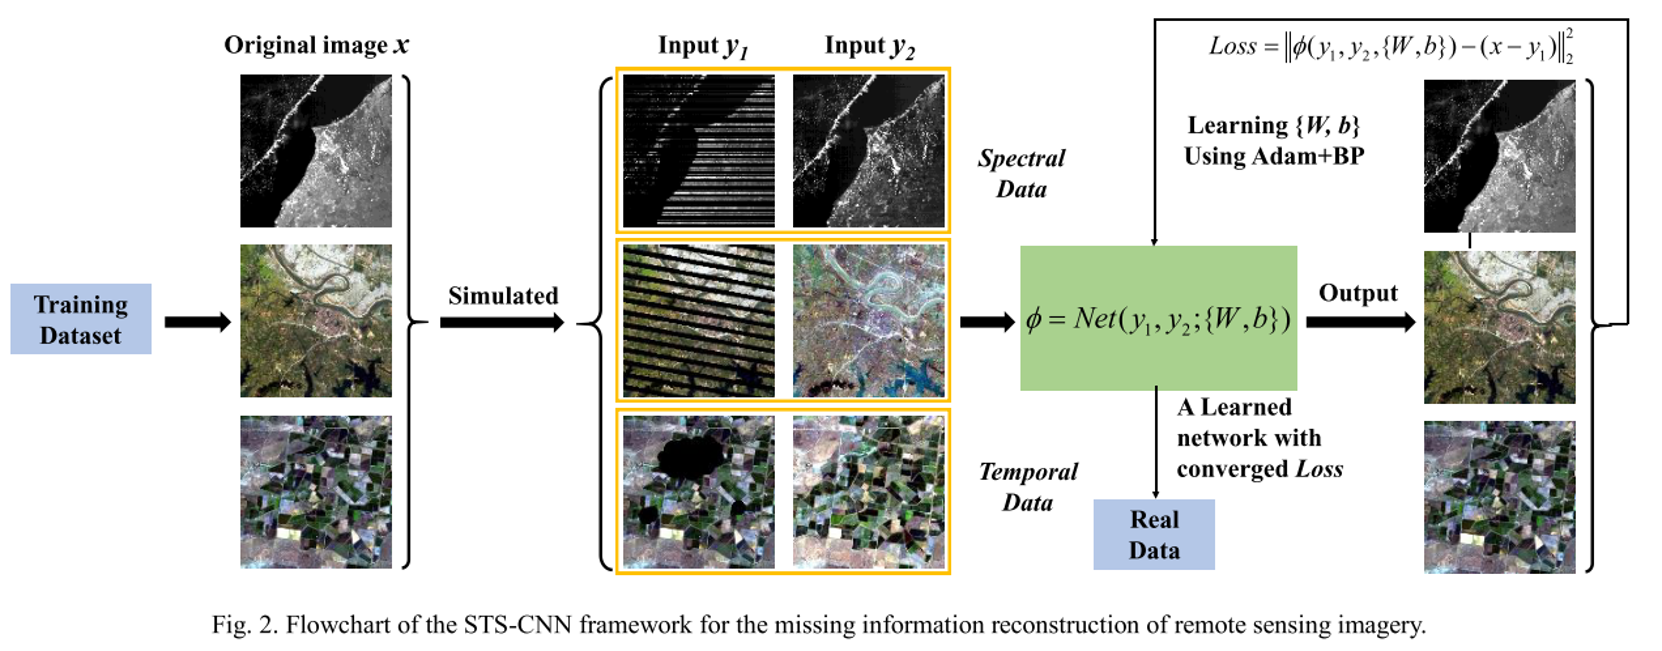
\includegraphics[width=1\textwidth]{figures/sts-cnn_framework.png}
	\caption{Flowchart of the STS-CNN framework in \cite{Zhang2018}}
\end{figure}

\section {Dataset}
In this chapter, Tri An reservoir is chosen for experiments, because it has enough large area for visualization, segmentation and calculation. Each tile from satellite imagery can only focus on part of the Earth, and Tri An reservoirs' water body belongs to one tile, so that it is not necessary to concatenate many tiles.

\begin{figure}[]
	\centering
	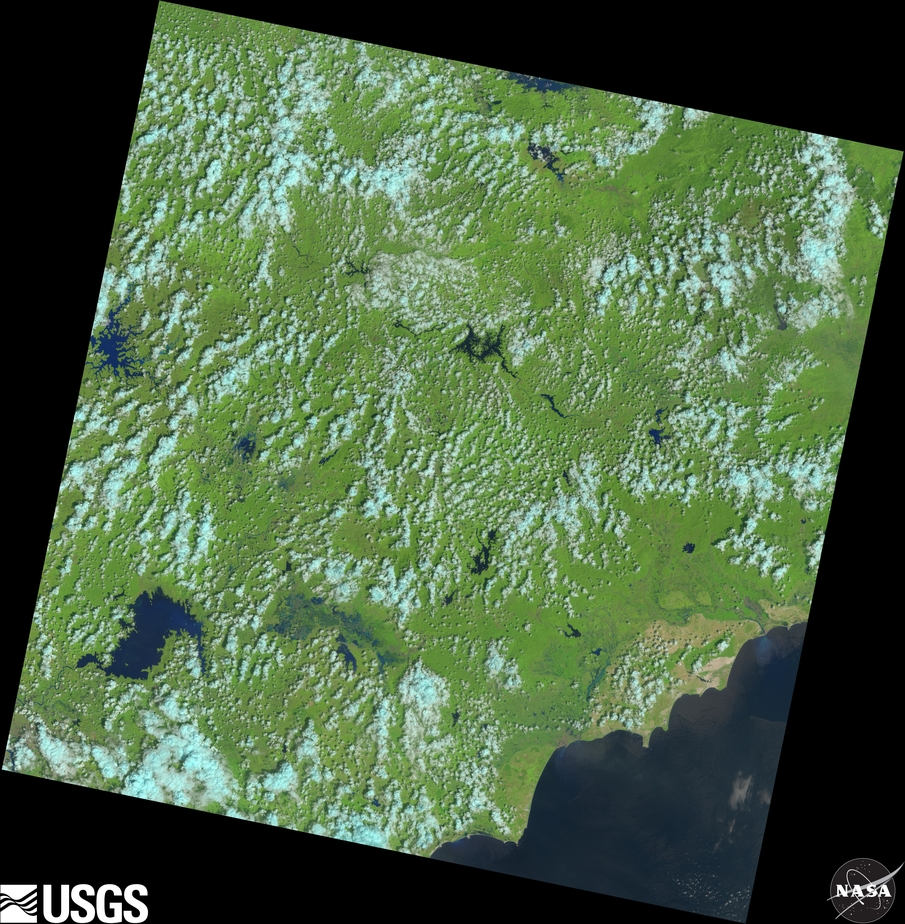
\includegraphics[width=0.4\textwidth]{figures/l8tile.png}
	\caption{Tri An Reservoir belongs to a tile of Landsat 8 data file, taken on January 10, 2013}
\end{figure}	


We use Landsat 8 data for optical satellite. For radar satellite, Sentinel-1 images are chosen. Those data can be freely acquired from the Internet.

\subparagraph{Requiring time period} \textbf{Landsat 8} data files are collected in period November 2013 - May 2018. SAR Imagery from \textbf{Sentinel-1} are from April 2014 - May 2018.

\section{Model}

In this method, we will refer a neural network of STS-CNN\cite{Zhang2018} to re-implement a neural network to our data. 

This algorithm has 3 inputs: (1) A missing image, (2) a referenced image and a missing image (1) with damaged regions filled by corresponding region in referenced image. The output is a recovered image. Note that, we have three images as input, and the third aims to tell a neural network easier to determine which are missing regions on the images. The referenced image will be also taken from Landsat 8, on cloudy-free day. For equal comparison to original method, we will use example of masks that provided with this paper, can be found at: \href{https://github.com/WHUQZhang/STS-CNN/}{https://github.com/WHUQZhang/STS-CNN/}.

The optimizer function is $Adam$ and the learning rate of whole network is $1e-4$. Model at figure \ref{fig:modifiedModel} contains 3 inputs: \textit{Input 1}: damaged image, \textit{Input 2}: referenced image and \textit{Input 3}: referenced with simulated-missing regions like \textit{Input 1}.

\begin{figure}[t]
	\centering
	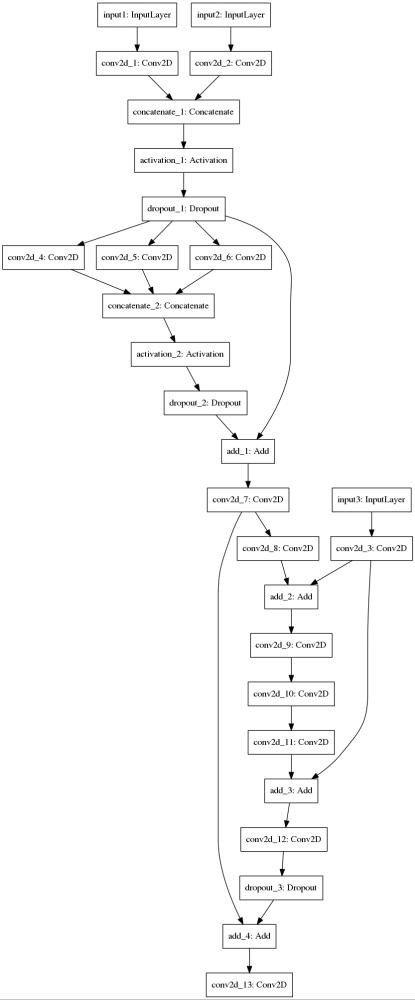
\includegraphics[width=0.6\textwidth]{figures/modifiedModel.png}
	\caption{Modified model from STS-CNN.}
	\label{fig:modifiedModel}
\end{figure}	

For comparison, we will use cloud-free image and add on it two type mask to feed into network. The first type is a simple shape mask from original method. The second is get from QA Bands of one cloud day, which is acquired by Landsat 8. In order to get cloud cover, F-mask program (Python, \href{http://pythonfmask.org}{http://pythonfmask.org}) is used to get cloud mask from QA Bands. The table shows difference between original method and my re-implemented method. For more visualization, take a look at figure \ref{fig:improvedModel_experiment_1}, \ref{fig:improvedModel_experiment_2} and \ref{fig:improvedModel_experiment_3} in \ref{experiment_improvedModel}. For measuring between methods, in this chapter, we use Peak signal-to-noise ratio.

\subparagraph{Peak signal-to-noise ratio} \textit{Wikipedia} It often abbreviated $PSNR$, is an engineering term for the ratio between the maximum possible power of a signal and the power of corrupting noise that affects the fidelity of its representation. Because many signals have a very wide dynamic range, $PSNR$ is usually expressed in terms of the logarithmic decibel scale. 

\begin{equation}
\centering
PSNR \textrm{ = } 20 * log_{10}(MAX_I) - 10 * log_{10}(MSE)
\end{equation}

where $MAX_I$ is the maximum possible value of image $I$, depending on its depth. For example, if the pixels are represented using 8 bits per sample ($8-bit$ image), this is 255. More generally, when samples are represented using linear PCM with $B$ bits per sample, $MAX_I$ is $2^B$ $-$ $1$. \textit{Mean square error}, $MSE$, between the original image $I$ with predicted image $K$, with the same of size ($m, n$) will be calculated as following:

\begin{equation}
\centering
MSE \textrm{ = } \frac{1}{mn} \sum_{i \textrm{ = } 1}^{m} \sum_{j \textrm{ = } 1}^{n} [I_{i,j} - K_{i,j}]^2
\end{equation}

\vspace{0.3cm}
Table of comparison:

\begin{table}[]
	\centering
	\begin{tabular}{|c|c|c|c|}
		\hline
		& STS-CNN & \begin{tabular}[c]{@{}c@{}}Modified model \\ (0..1)\end{tabular} & \begin{tabular}[c]{@{}c@{}}Modified model \\ (0..255)\end{tabular} \\ \hline
		Simple cloud         & 19.9098 & \textbf{27.00188}                                                & 26.7391                                                            \\ \hline
		Simple multi-cloud   & 15.6941 & \textbf{23.8445}                                                 & 23.80995                                                           \\ \hline
		Real (complex) cloud & 12.8381 & \textbf{19.70776}                                                & 19.5976                                                            \\ \hline
	\end{tabular}
	\caption{Comparison between proposed model to modified model. Pixel value are scale to $(0..1)$ and $(0..255)$ (original has pixel range from $0..65535$). All are calculated by $PSNR$. Higher is better}
\end{table}

\section{Optimization}

As periodicity of weather is being used for higher accuracy in recovering water body, we use two methods below on our dataset: (1) \textbf{Using Time-Distributed Layer from Keras}; (2) \textbf{Recurrent-CNN}, which uses a kind of Recurrent Neural Network, Long-Short Term Memory. A common thing between between two approaches is applying a temporal slice of images into neural network, and the purpose of those sub-networks is predicting the next images to be referenced image. 

\subsection{Using Time-Distributed Layer from Keras}

Keras framework also provides Time-Distributed layers, which applies for every temporal slice of an input. Because of limitation of hardware memory, we feed into it five consecutive images acquired from Landsat 8. For referenced image, we try with 2 type: first is Landsat 8 and the second is Sentinel-1. Because only water body is focused, so we've classified water body on Sentinel-1 data, and resize it to the same of Landsat 8 (Sentinel-1 has 10 meters of resolution). Model specification contains 2 part: \textit{part 1}  (at Fig. \ref{fig:timemodelPart1}) is about using Time-Distributed to get predicted image as reference, \textit{part 2} (at Fig. \ref{fig:timemodelPart2}) is quite similar to existing method for reconstruction.

\begin{figure}[]
	\centering
	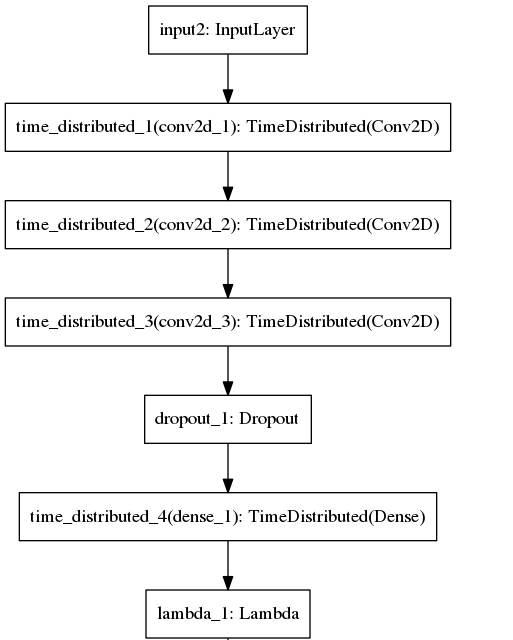
\includegraphics[width=0.5\textwidth]{figures/timemodelPart1.png}
	\caption{Applying Time-Distributed in Neural Network. Lambda is a function to get 1-time next predicted image from time-series images to be reference image.}
	\label{fig:timemodelPart1}
\end{figure}

\begin{figure}[]
	\centering
	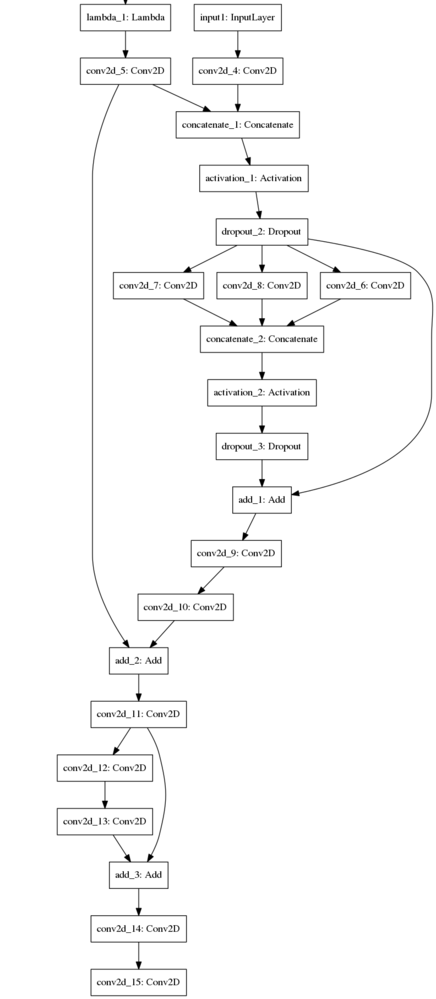
\includegraphics[width=0.7\textwidth]{figures/timemodelPart2.png}
	\caption{Using predicted image as reference image, with part in order to reconstruct missing regions. Note that there is not input \textit{referenced image with missing data}}
	\label{fig:timemodelPart2}
\end{figure}

\subsection{Recurrent-CNN implementation}

The idea behind Recurrent Neural Networks (RNNs) is to make use of sequential information. So that, this approach aims to use Long Short Term Memory networks – usually just called “LSTMs” – are a special kind of RNN, capable of learning long-term dependencies, to make prediction of next image, based on five consecutive images, and use the next image as referenced image for reconstruction. For the predictive part, see \ref{fig:modelConv2DLSTM_1}. The main is similar to \ref{fig:timemodelPart2}

\begin{figure}[]
	\centering
	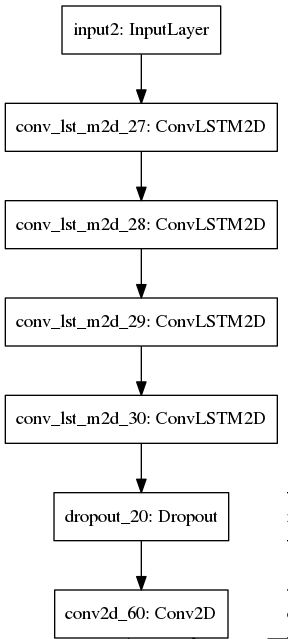
\includegraphics[width=0.5\textwidth]{figures/modelConv2DLSTM_1.png}
	\caption{LSTM (as Conv2DLSTM Layer) aims to predict the next image to be used as referenced image}
	\label{fig:modelConv2DLSTM_1}
\end{figure}

\subsection{Comparison}

This is a comparison between above methods. Visualization is available at \ref{experiment_timeSeriesModel}, in which \textit{Input 1 is damaged image, input 2 is a time-series data (5 images)}. 

\begin{table}[]
	\centering
	\begin{tabular}{|c|c|c|}
		\hline
		& \begin{tabular}[c]{@{}c@{}}Time-Distributed\\ Layers\end{tabular} & LSTM-Conv2D \\ \hline
		Simple cloud         & \textbf{30.5584}                                                  & 23.4441     \\ \hline
		Simple multi-cloud   & \textbf{29.9230}                                                  & 24.0554     \\ \hline
		Real (complex) cloud & \textbf{30.4467}                                                  & 26.4210     \\ \hline
	\end{tabular}
	\caption{Comparison when applying time-series images for predicting next image as reference.}
\end{table}

\section{Experiments}

\subsection{One reference image - Comparison with original method}\label{experiment_improvedModel}

In this section, we take an example from testing data. Band 3, 4, 5 \textit{(Red, Green, Near IR from Landsat 8)} were chosen for making RGB image. For image within range $0..1$, after reconstructed, we multiply for each pixel by 255.
\begin{figure}[]
	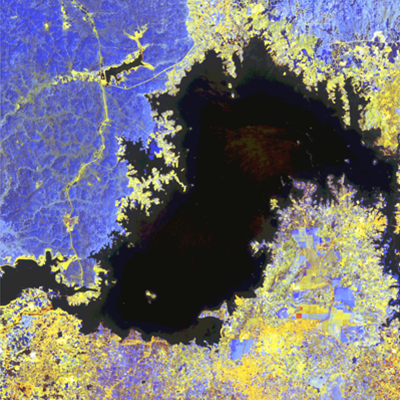
\includegraphics[width=0.7\linewidth]{figures/groud_truth.png}
	\centering
	\caption{Ground Truth}
\end{figure}

\subsubsection{Easiest case: Simple cloud shape}

\begin{figure}[]
	\centering
	\subfloat[]{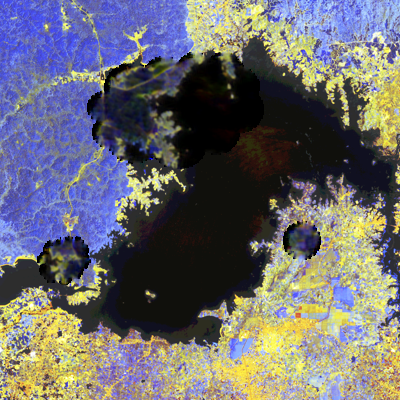
\includegraphics[width=0.32\linewidth]{figures/sts_sample_cloud.png}}
	\subfloat[]{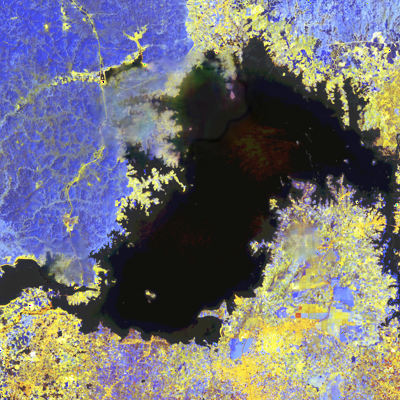
\includegraphics[width=0.32\linewidth]{figures/1_simple.png}}
	\subfloat[]{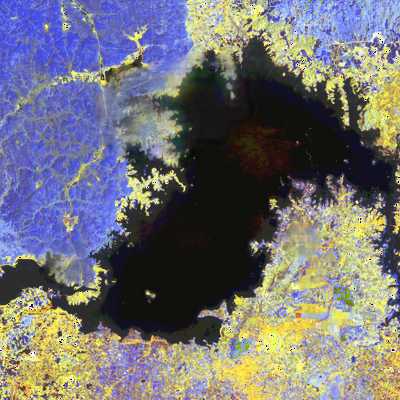
\includegraphics[width=0.32\linewidth]{figures/255_simple.png}} 
	\centering
	\caption{
		\textbf{(a)} STS-CNN.
		\textbf{(b)} Modified Model, range $0..1$.
		\textbf{(c)} Modified Model, range $0..255$}
	\label{fig:improvedModel_experiment_1}
\end{figure}


\subsubsection{Average case: Multi-simple cloud shape}

\begin{figure}[]
	\centering
	\subfloat[]{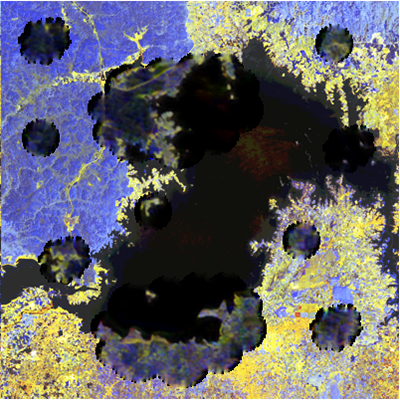
\includegraphics[width=0.32\linewidth]{figures/sts_sample_multicloud.png}}
	\subfloat[]{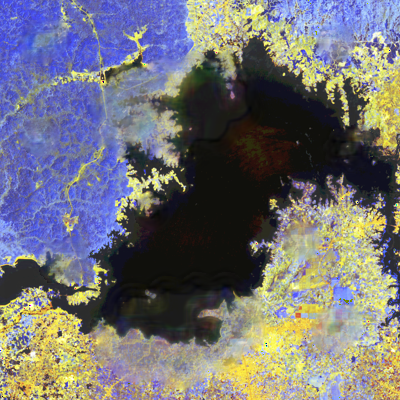
\includegraphics[width=0.32\linewidth]{figures/1_multiFake.png}}
	\subfloat[]{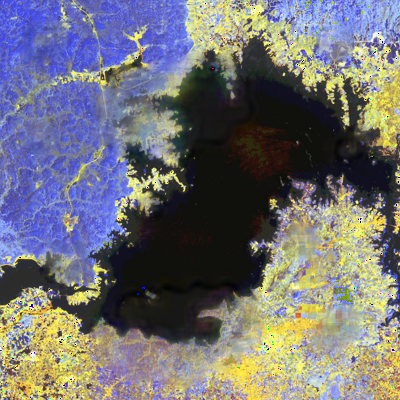
\includegraphics[width=0.32\linewidth]{figures/255_multi_fake.png}} 
	\centering
	\caption{
		\textbf{(a)} STS-CNN.
		\textbf{(b)} Modified Model, range $0..1$.
		\textbf{(c)} Modified Model, range $0..255$}
	\label{fig:improvedModel_experiment_2}
\end{figure}

\subsubsection{Hardest case: Real cloud}

\begin{figure}[]
	\centering
	\subfloat[]{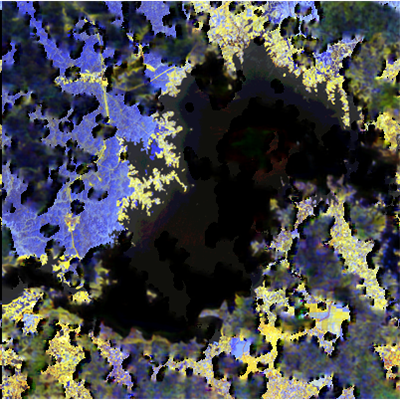
\includegraphics[width=0.32\linewidth]{figures/sts_real_cloud.png}}
	\subfloat[]{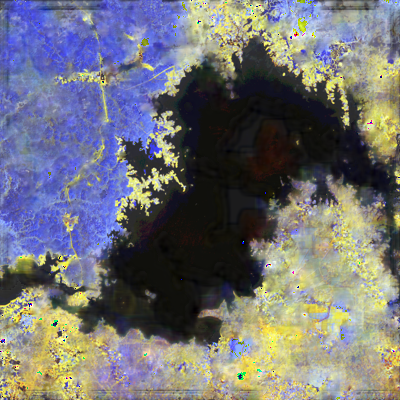
\includegraphics[width=0.32\linewidth]{figures/1_complex.png}}
	\subfloat[]{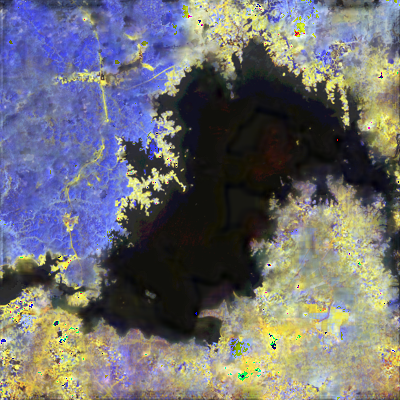
\includegraphics[width=0.32\linewidth]{figures/255_complex.png}} 
	\centering
	\caption{
		\textbf{(a)} STS-CNN.
		\textbf{(b)} Modified Model, range $0..1$.
		\textbf{(c)} Modified Model, range $0..255$}
	\label{fig:improvedModel_experiment_3}
\end{figure}


\subsection{Trying to recover water body}\label{experiment_timeSeriesModel}
Model has been trained in \textbf{4.1} to take experiments on recovering water body from reconstructed images in cloud days. In order to recover water body, images are collected from Landsat 8 will be crop to be size of $1200 x 1600$ pixels, equals $3 x 4$ tiles, each tiles has size of $400 x 400$ pixels.  

For segmentation, NDWI-index is used to mask out water body. For comparison to ground truth, the most nearest SAR-image collected from Sentinel-1 will be used. 

All Landsat 8 images has been calculated by NDWI formula:

\begin{equation}
NDWI = \frac{Green - Near IR}{Green + Near IR}
\end{equation}

and the display images only contain pixel that having NDWI-index above 0 (which are water or cloud pixel). For Sentinel-1 images, VH-band is used. The pixel belongs to water have value less than -22.

\subparagraph{Explanation for figures} Note that, \textbf{(a)} is covered by cloud, \textbf{(b)} is recovered and \textbf{(c)} is collected from Sentinel-1. 

\begin{figure}[]
	\centering
	\subfloat[60.6114 $km^2$]{
		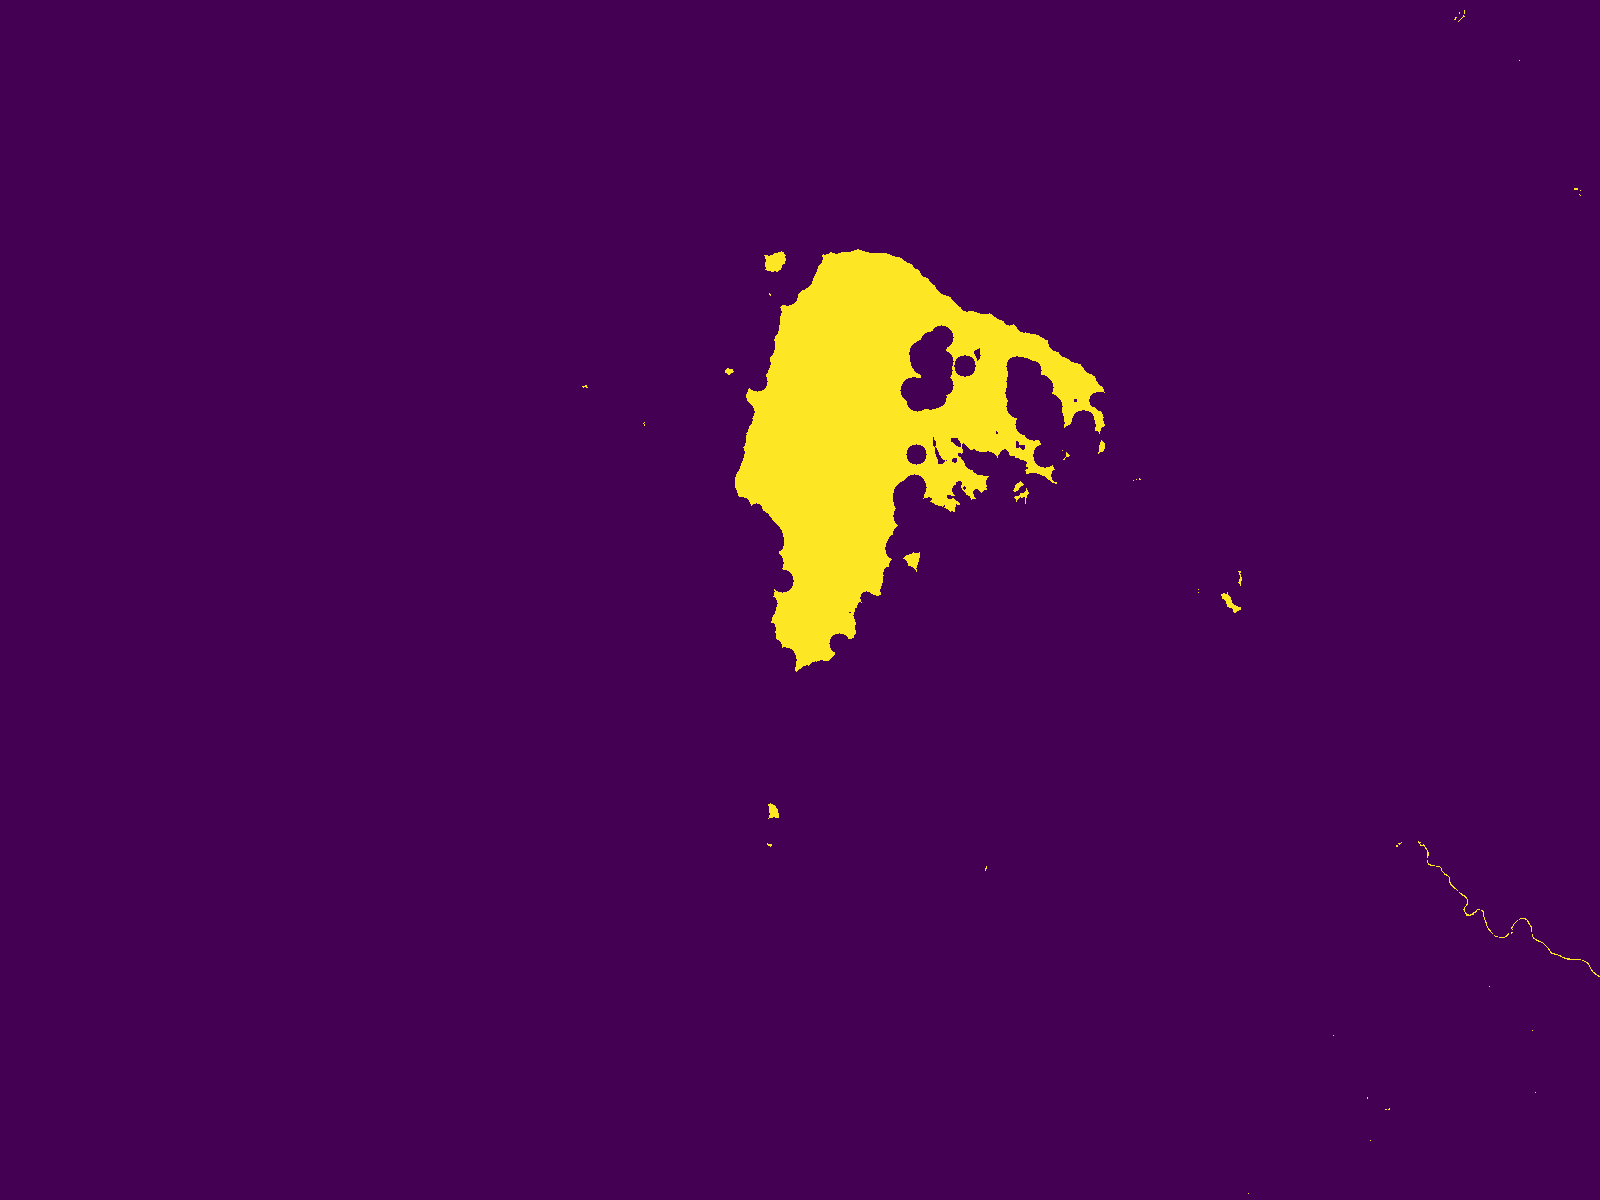
\includegraphics[width=0.32\linewidth]{figures/raw20160104_60_6114.png}
	}
	\subfloat[242.0488 $km^2$]{
		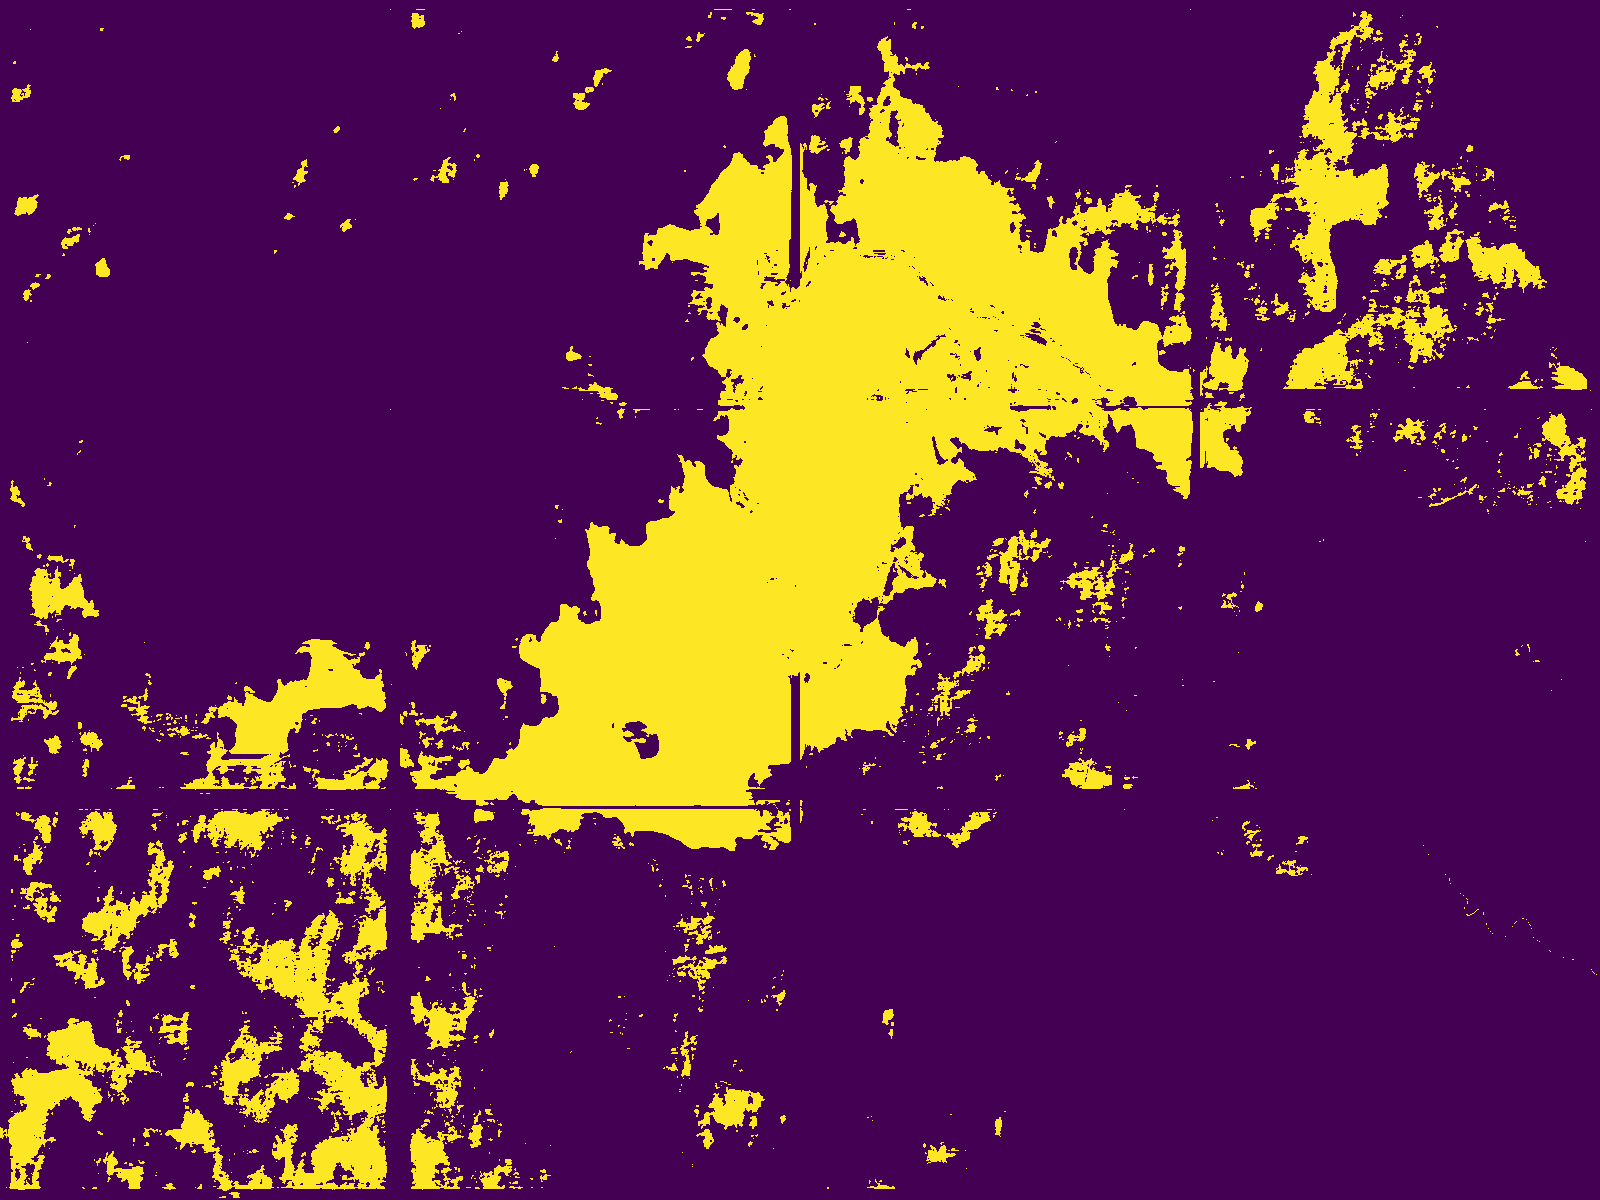
\includegraphics[width=0.32\linewidth]{figures/r20160104_242_0488.png}
	}
	\subfloat[269.2041 $km^2$]{
		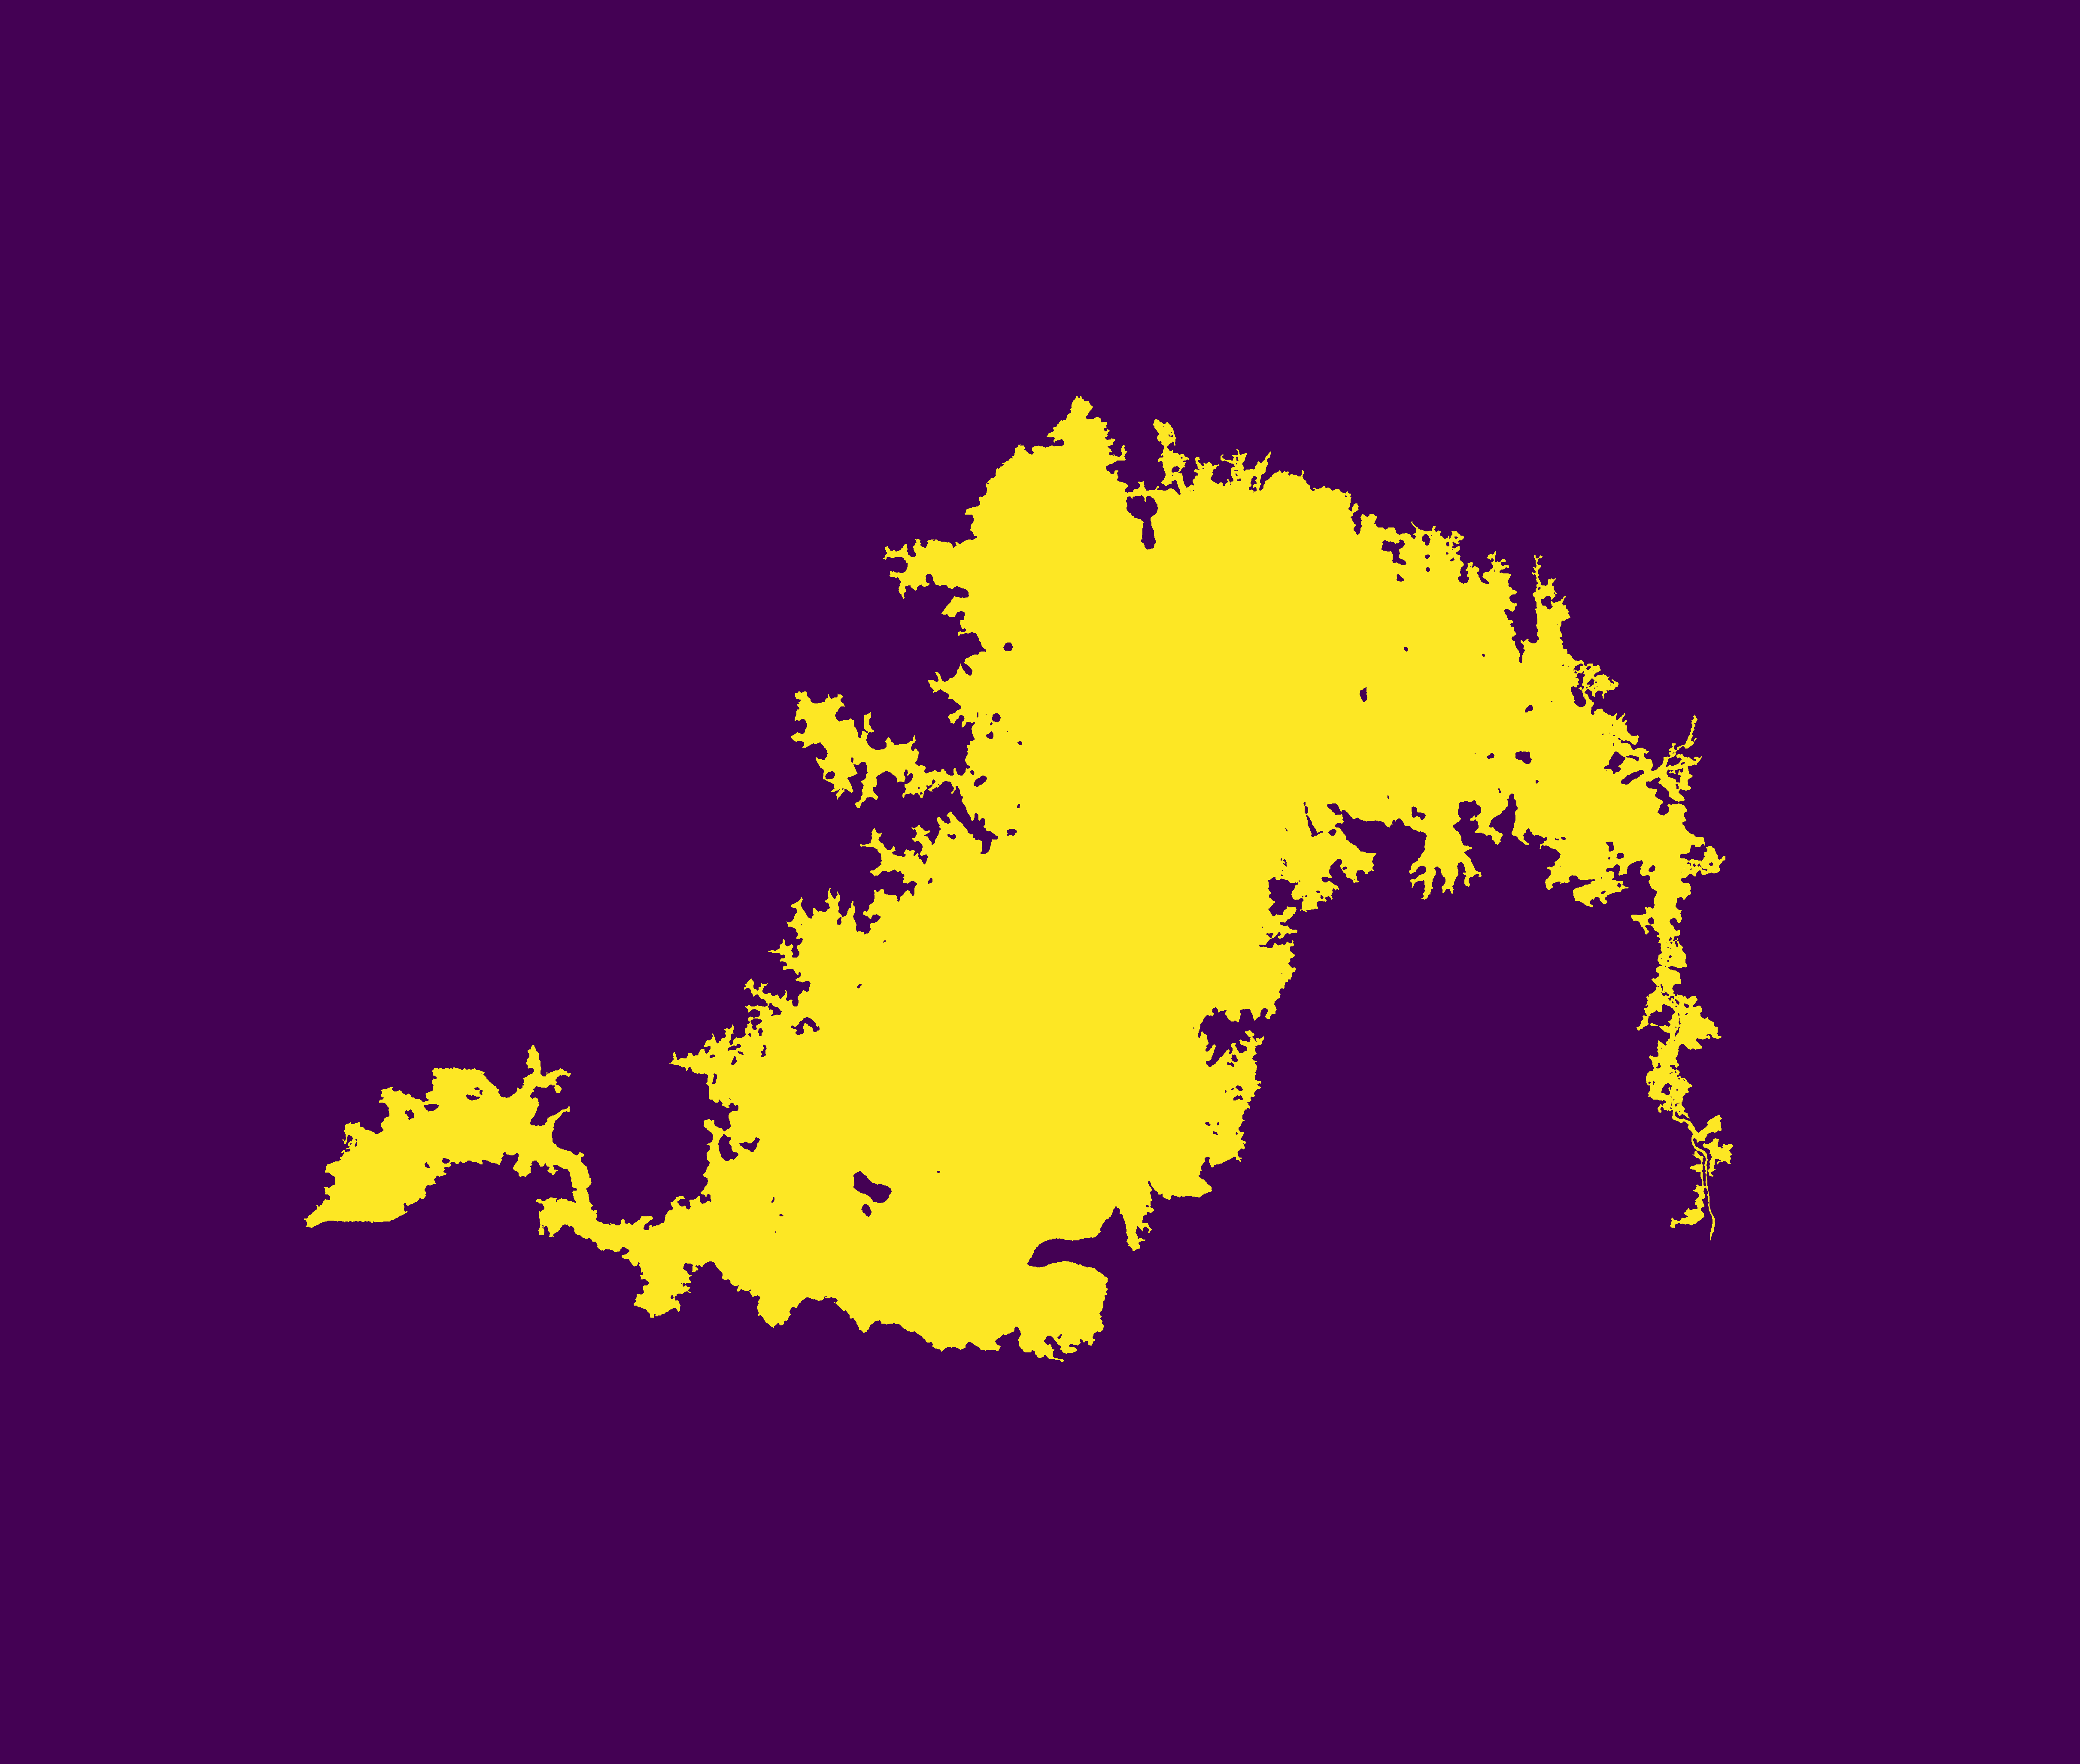
\includegraphics[width=0.32\linewidth]{figures/20160112_269_2041.png}
	} 
	\centering
	\caption{
		\textbf{(a, b)} Landsat 8, Jan 4th 2016.
		\textbf{(c)} Sentinel-1, Jan 12th 2016.}
\end{figure}


\begin{figure}[]
	\centering
	\subfloat[51.8346 $km^2$]{
		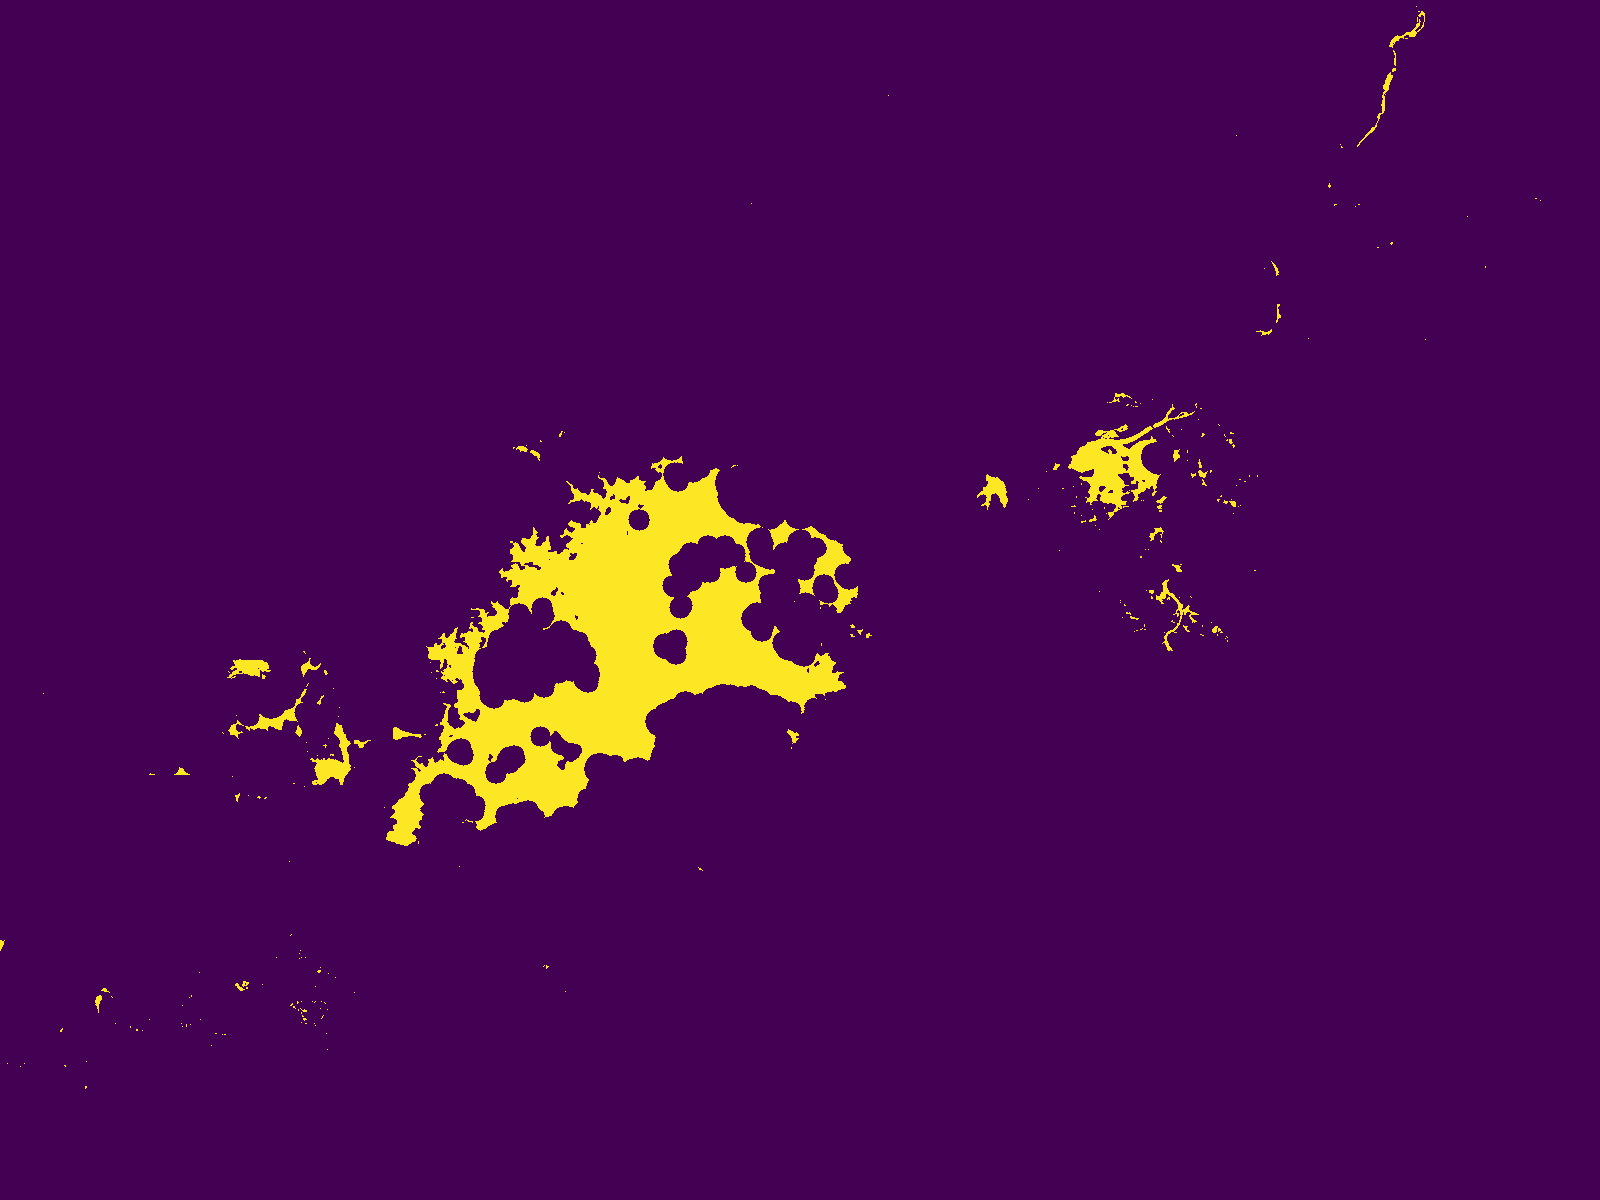
\includegraphics[width=0.32\linewidth]{figures/raw20160815_51_8346.png}
	}
	\subfloat[193.9509 $km^2$]{
		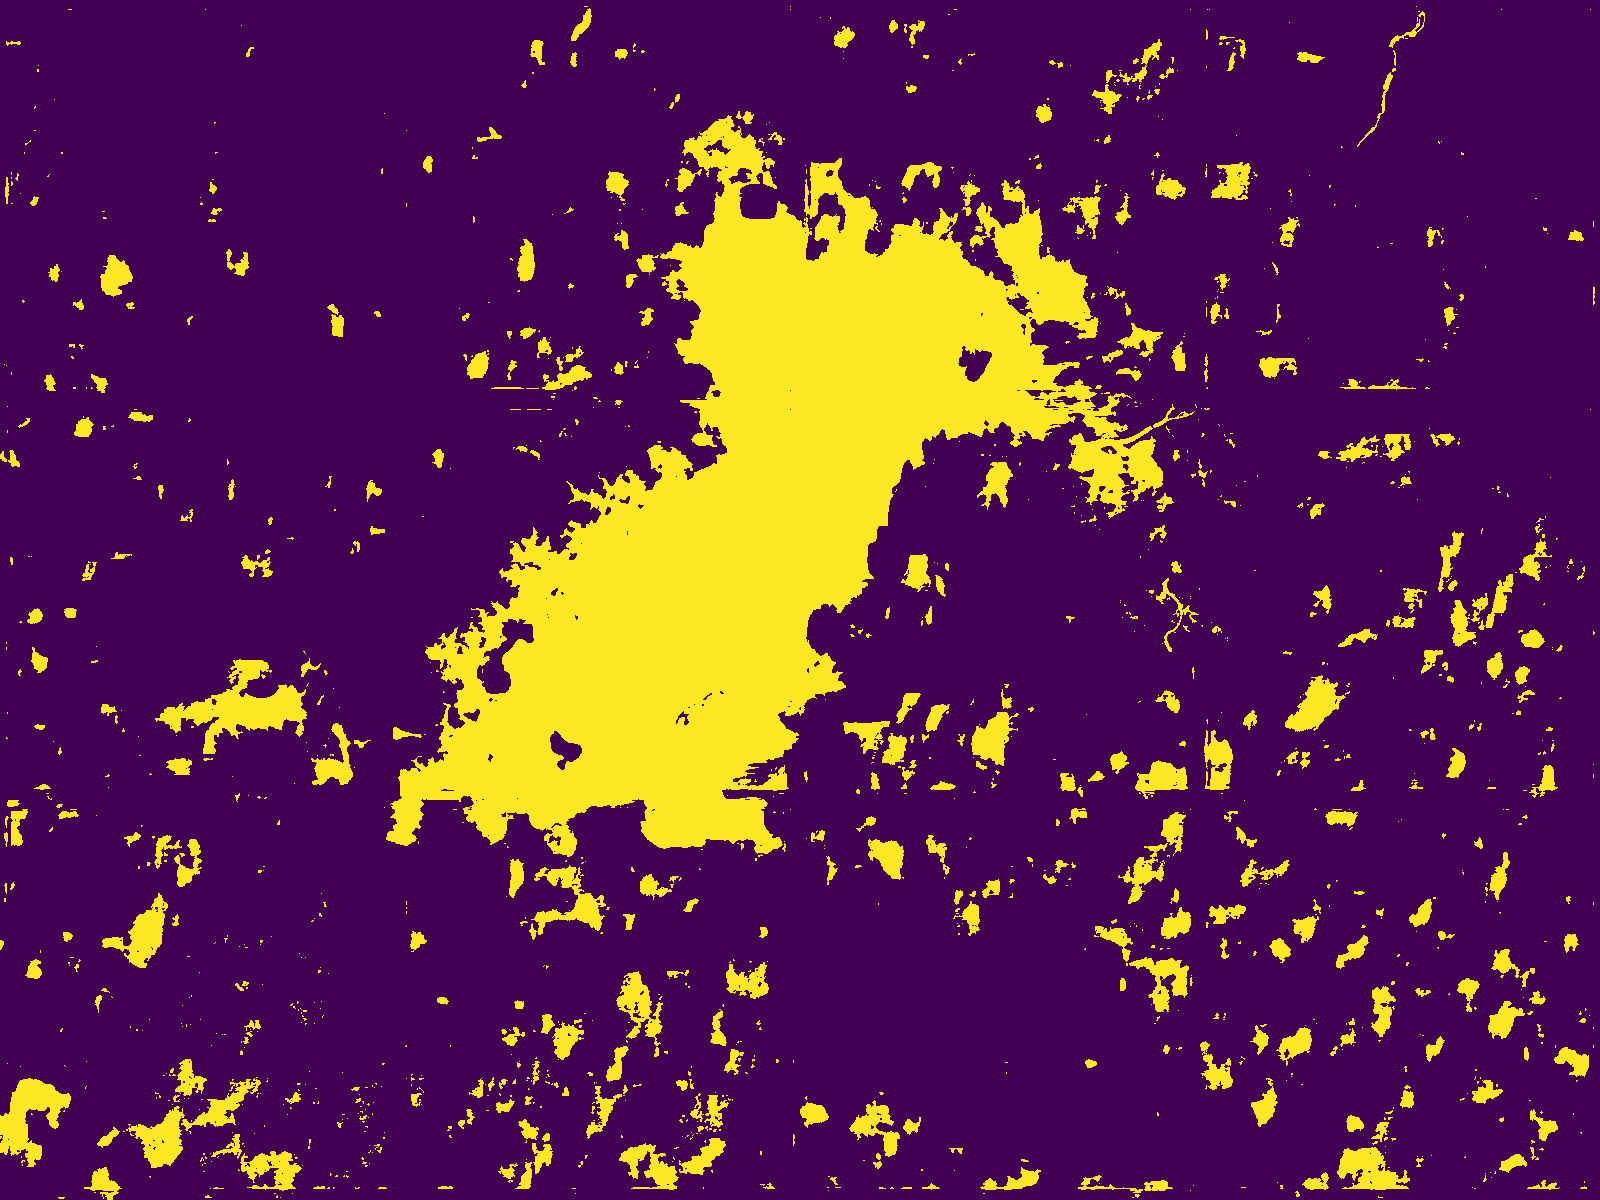
\includegraphics[width=0.32\linewidth]{figures/r20160815_193_9509.png}
	}
	\subfloat[201.6019 $km^2$]{
		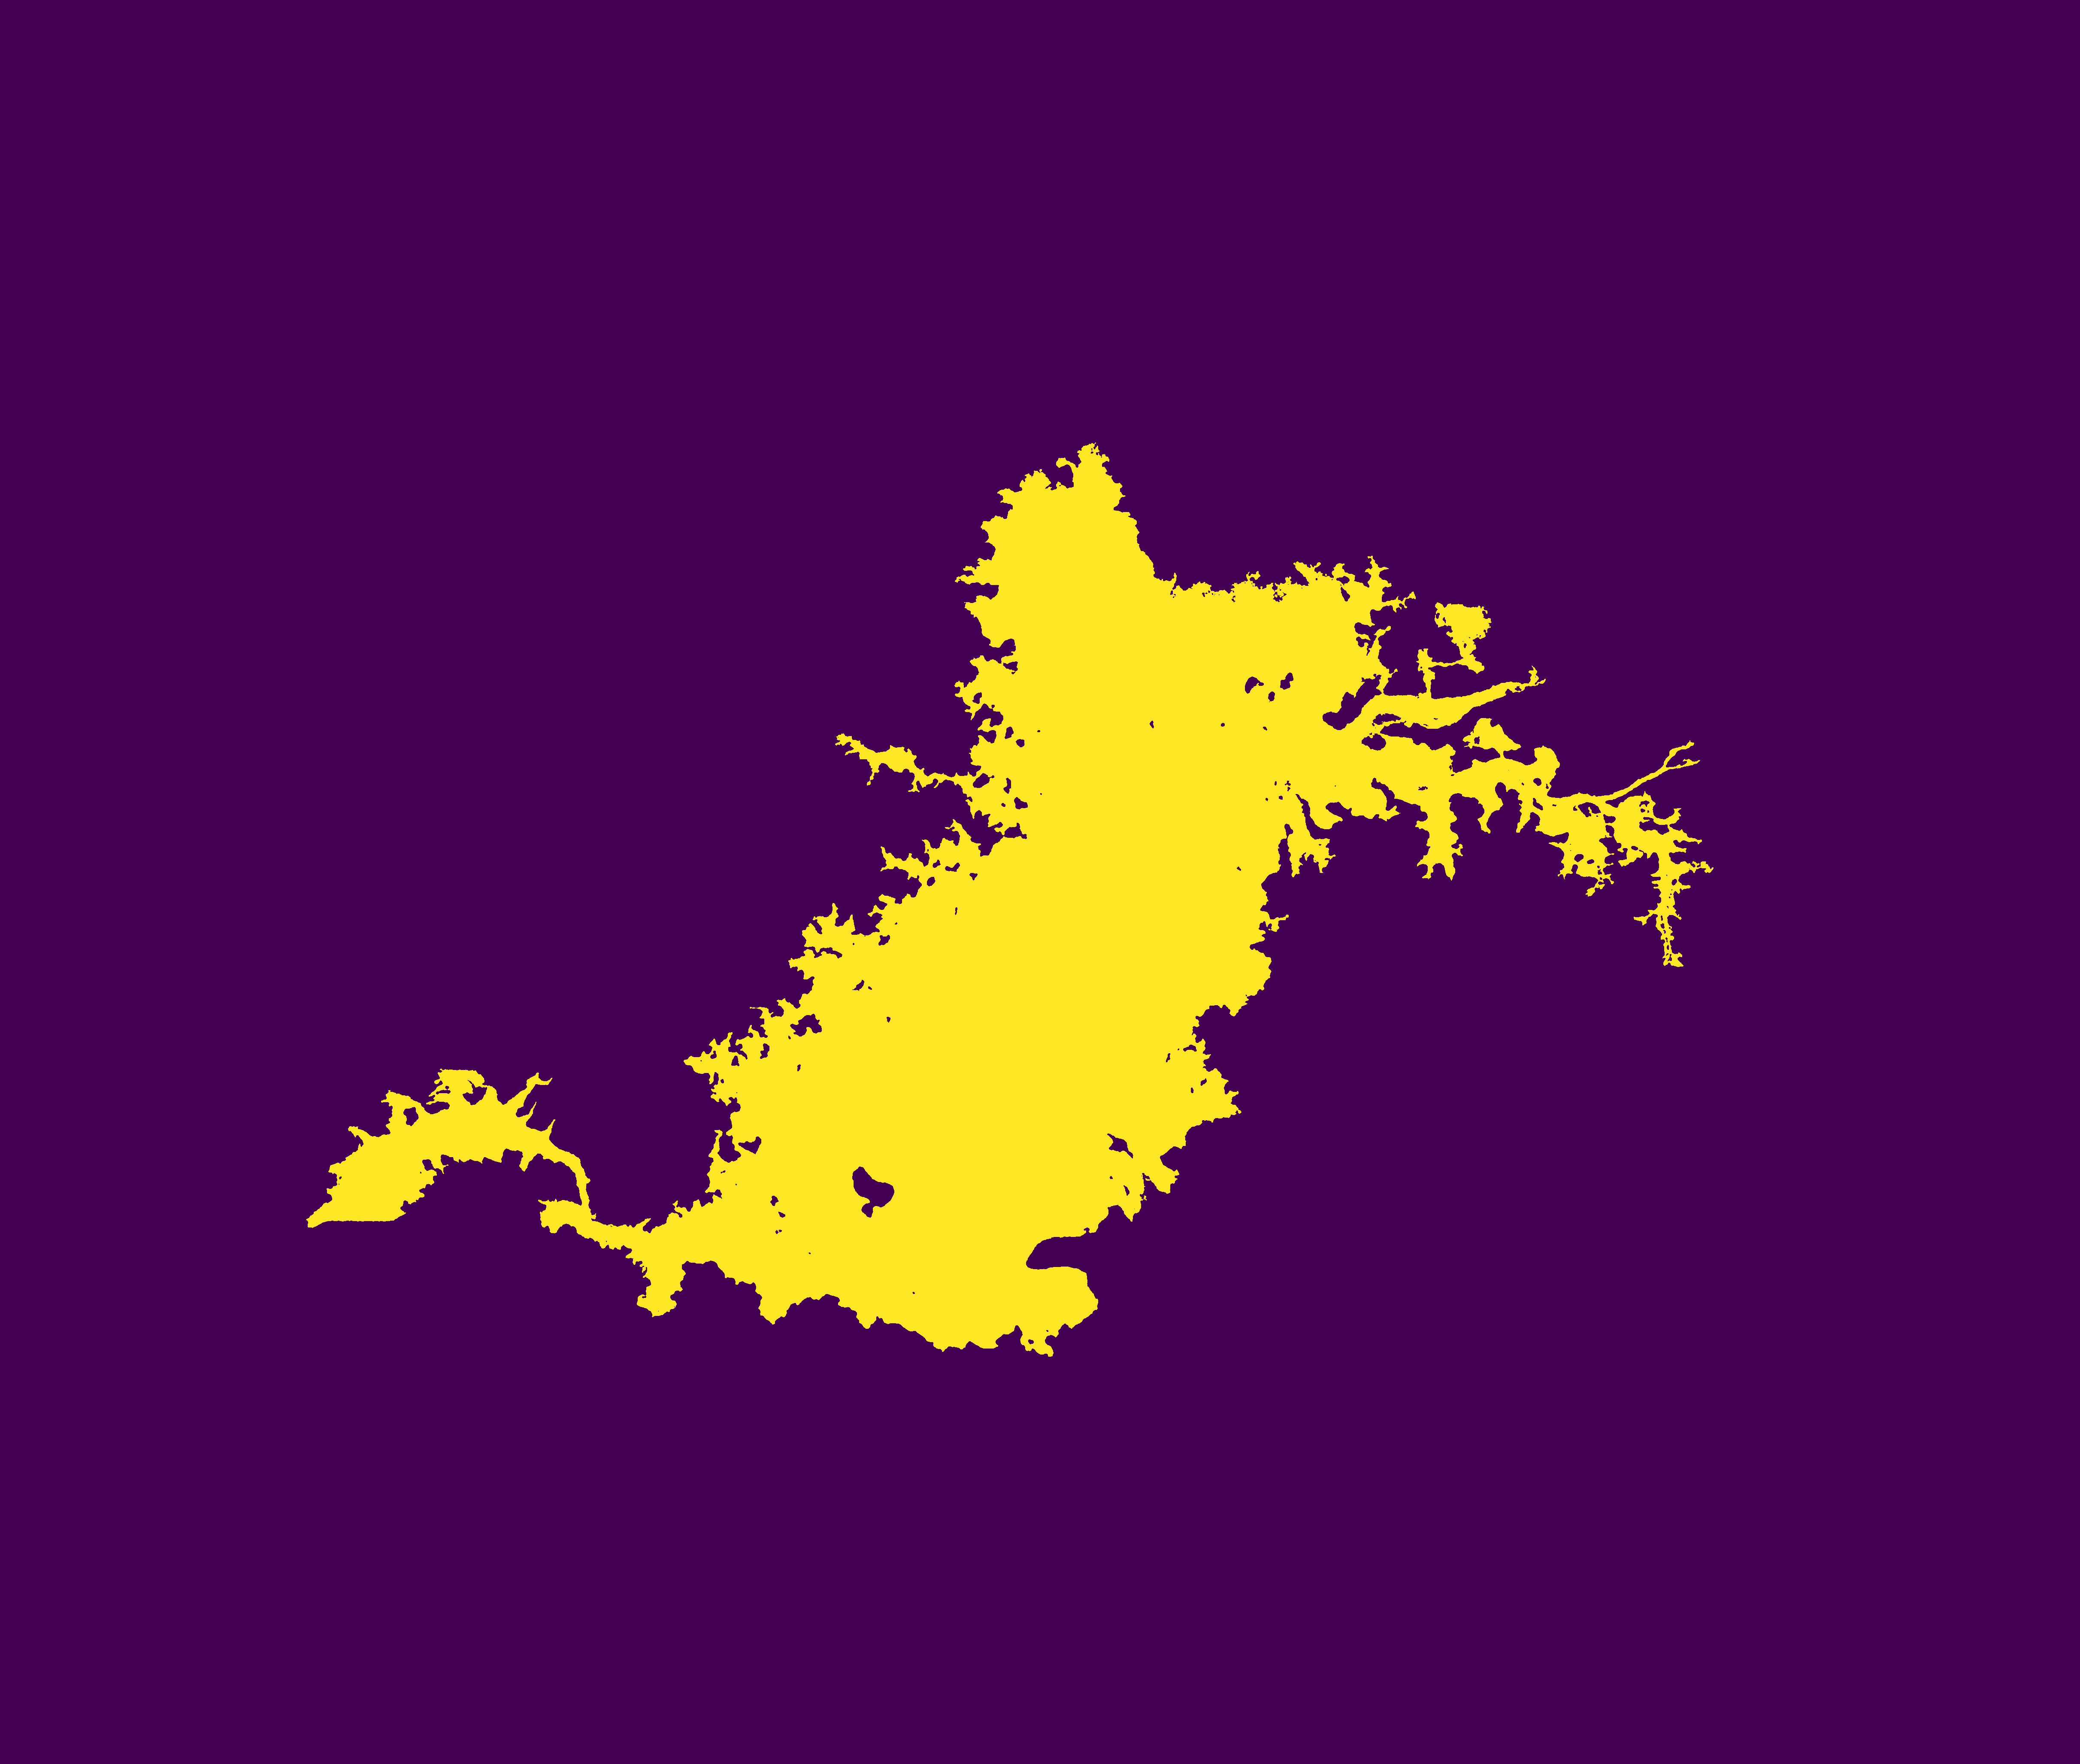
\includegraphics[width=0.32\linewidth]{figures/20160815_201_6019.png}
	} 
	
	\centering
	\caption{
		\textbf{(a, b)} Landsat 8, Aug 15th 2016.
		\textbf{(c)} Sentinel-1, Aug 15th 2016.}
	\end{figure}


\begin{figure}[]
\centering
\subfloat[31.2336 $km^2$]{
	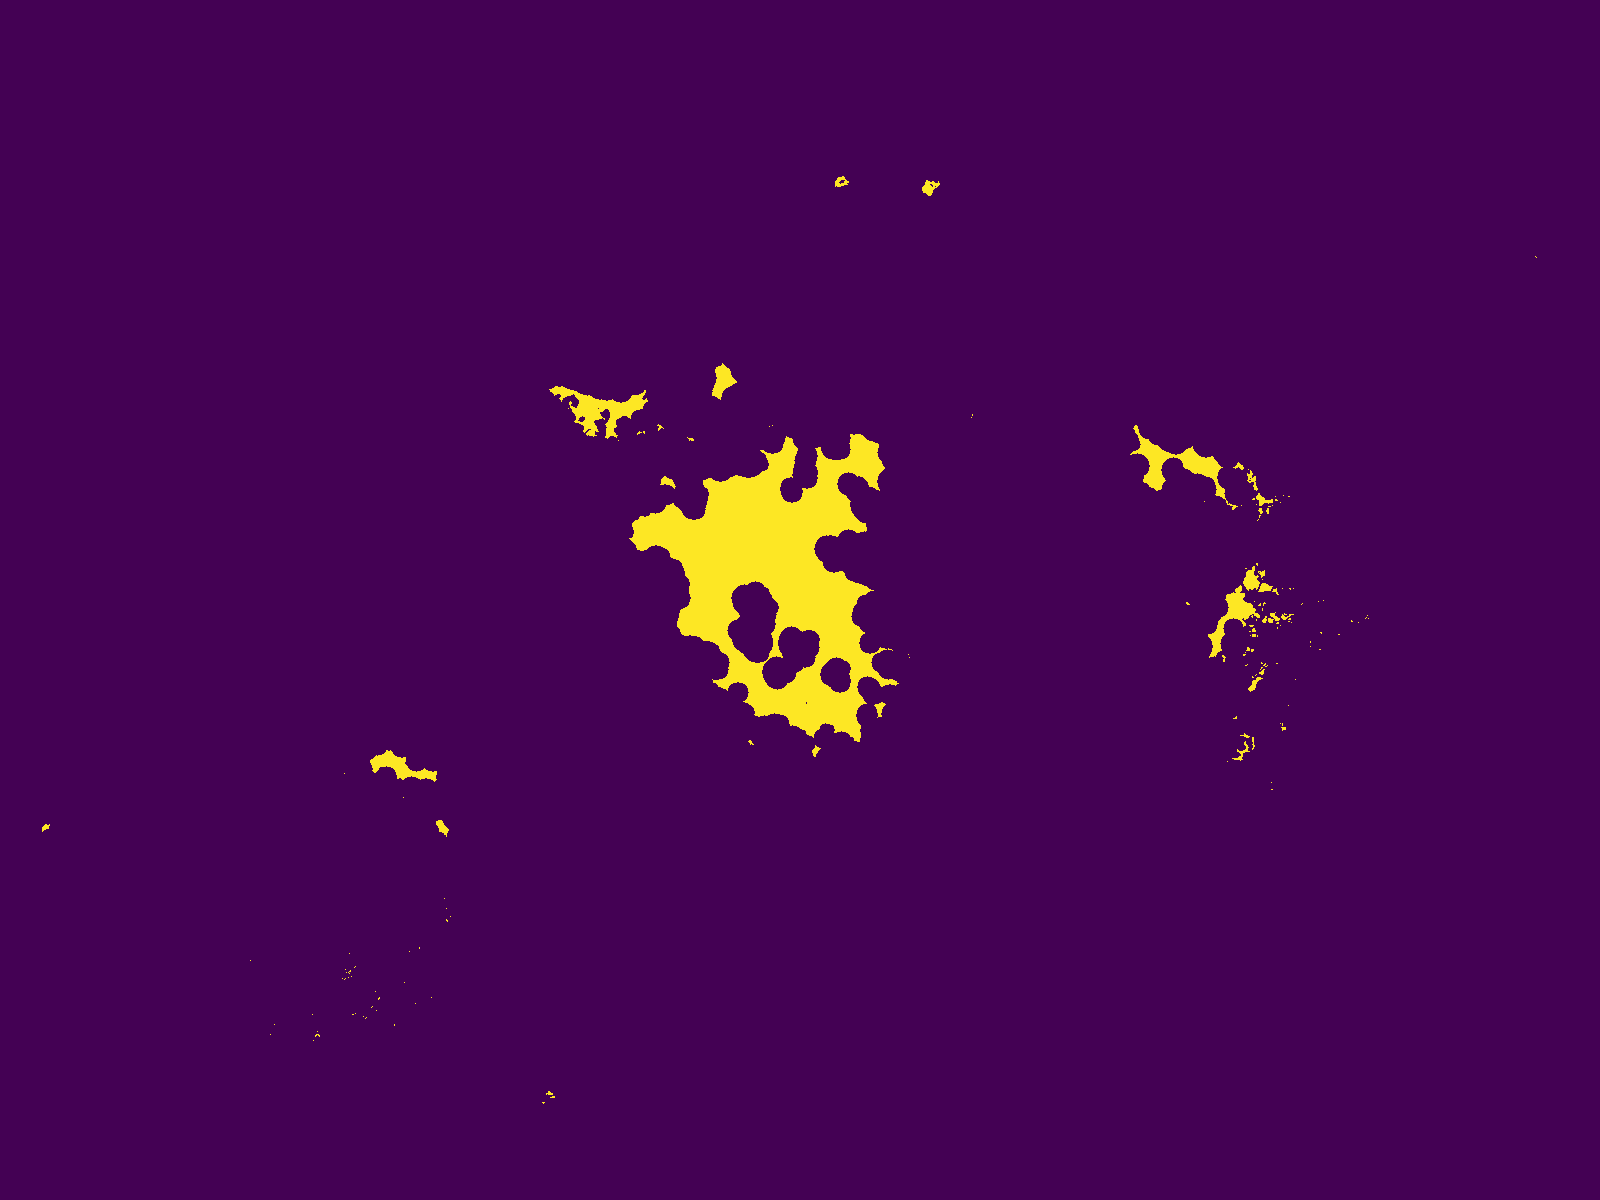
\includegraphics[width=0.32\linewidth]{figures/raw20170802_31_2336.png}
}
\subfloat[185.7141 $km^2$]{
	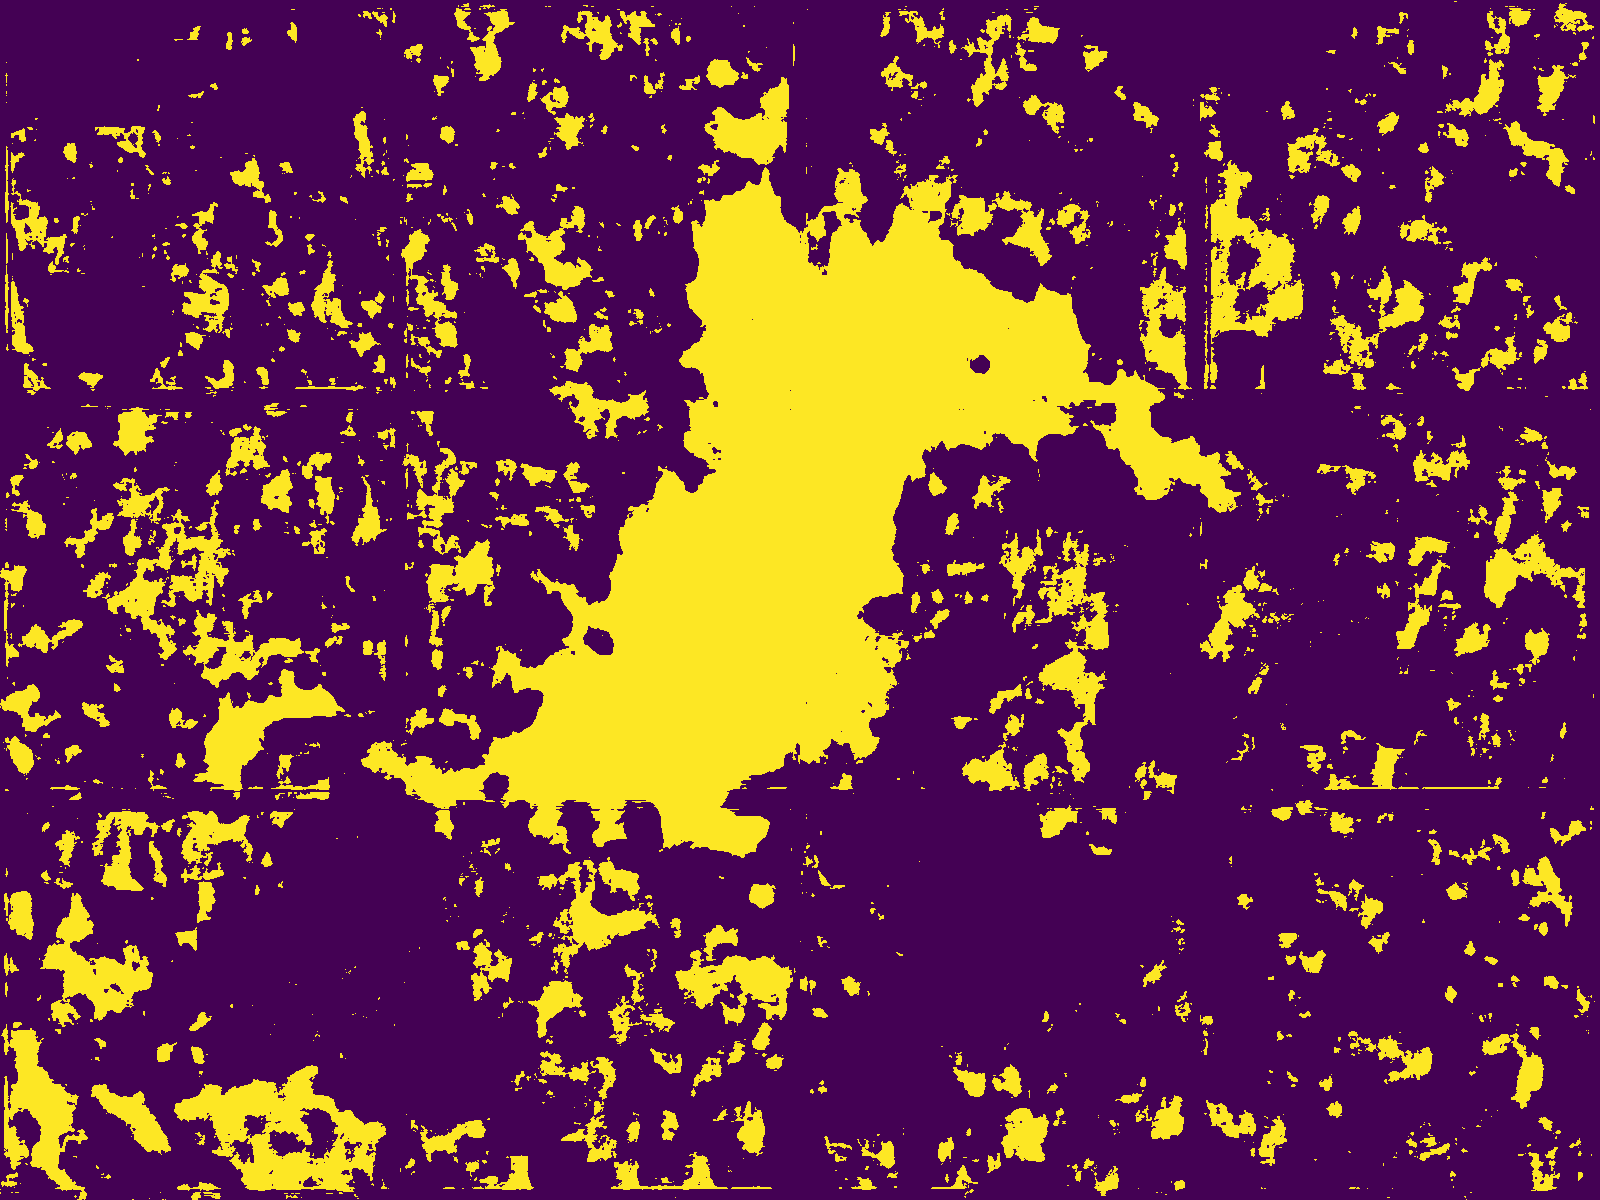
\includegraphics[width=0.32\linewidth]{figures/r20170802_185_7141.png}
}
\subfloat[258.6828 $km^2$]{
	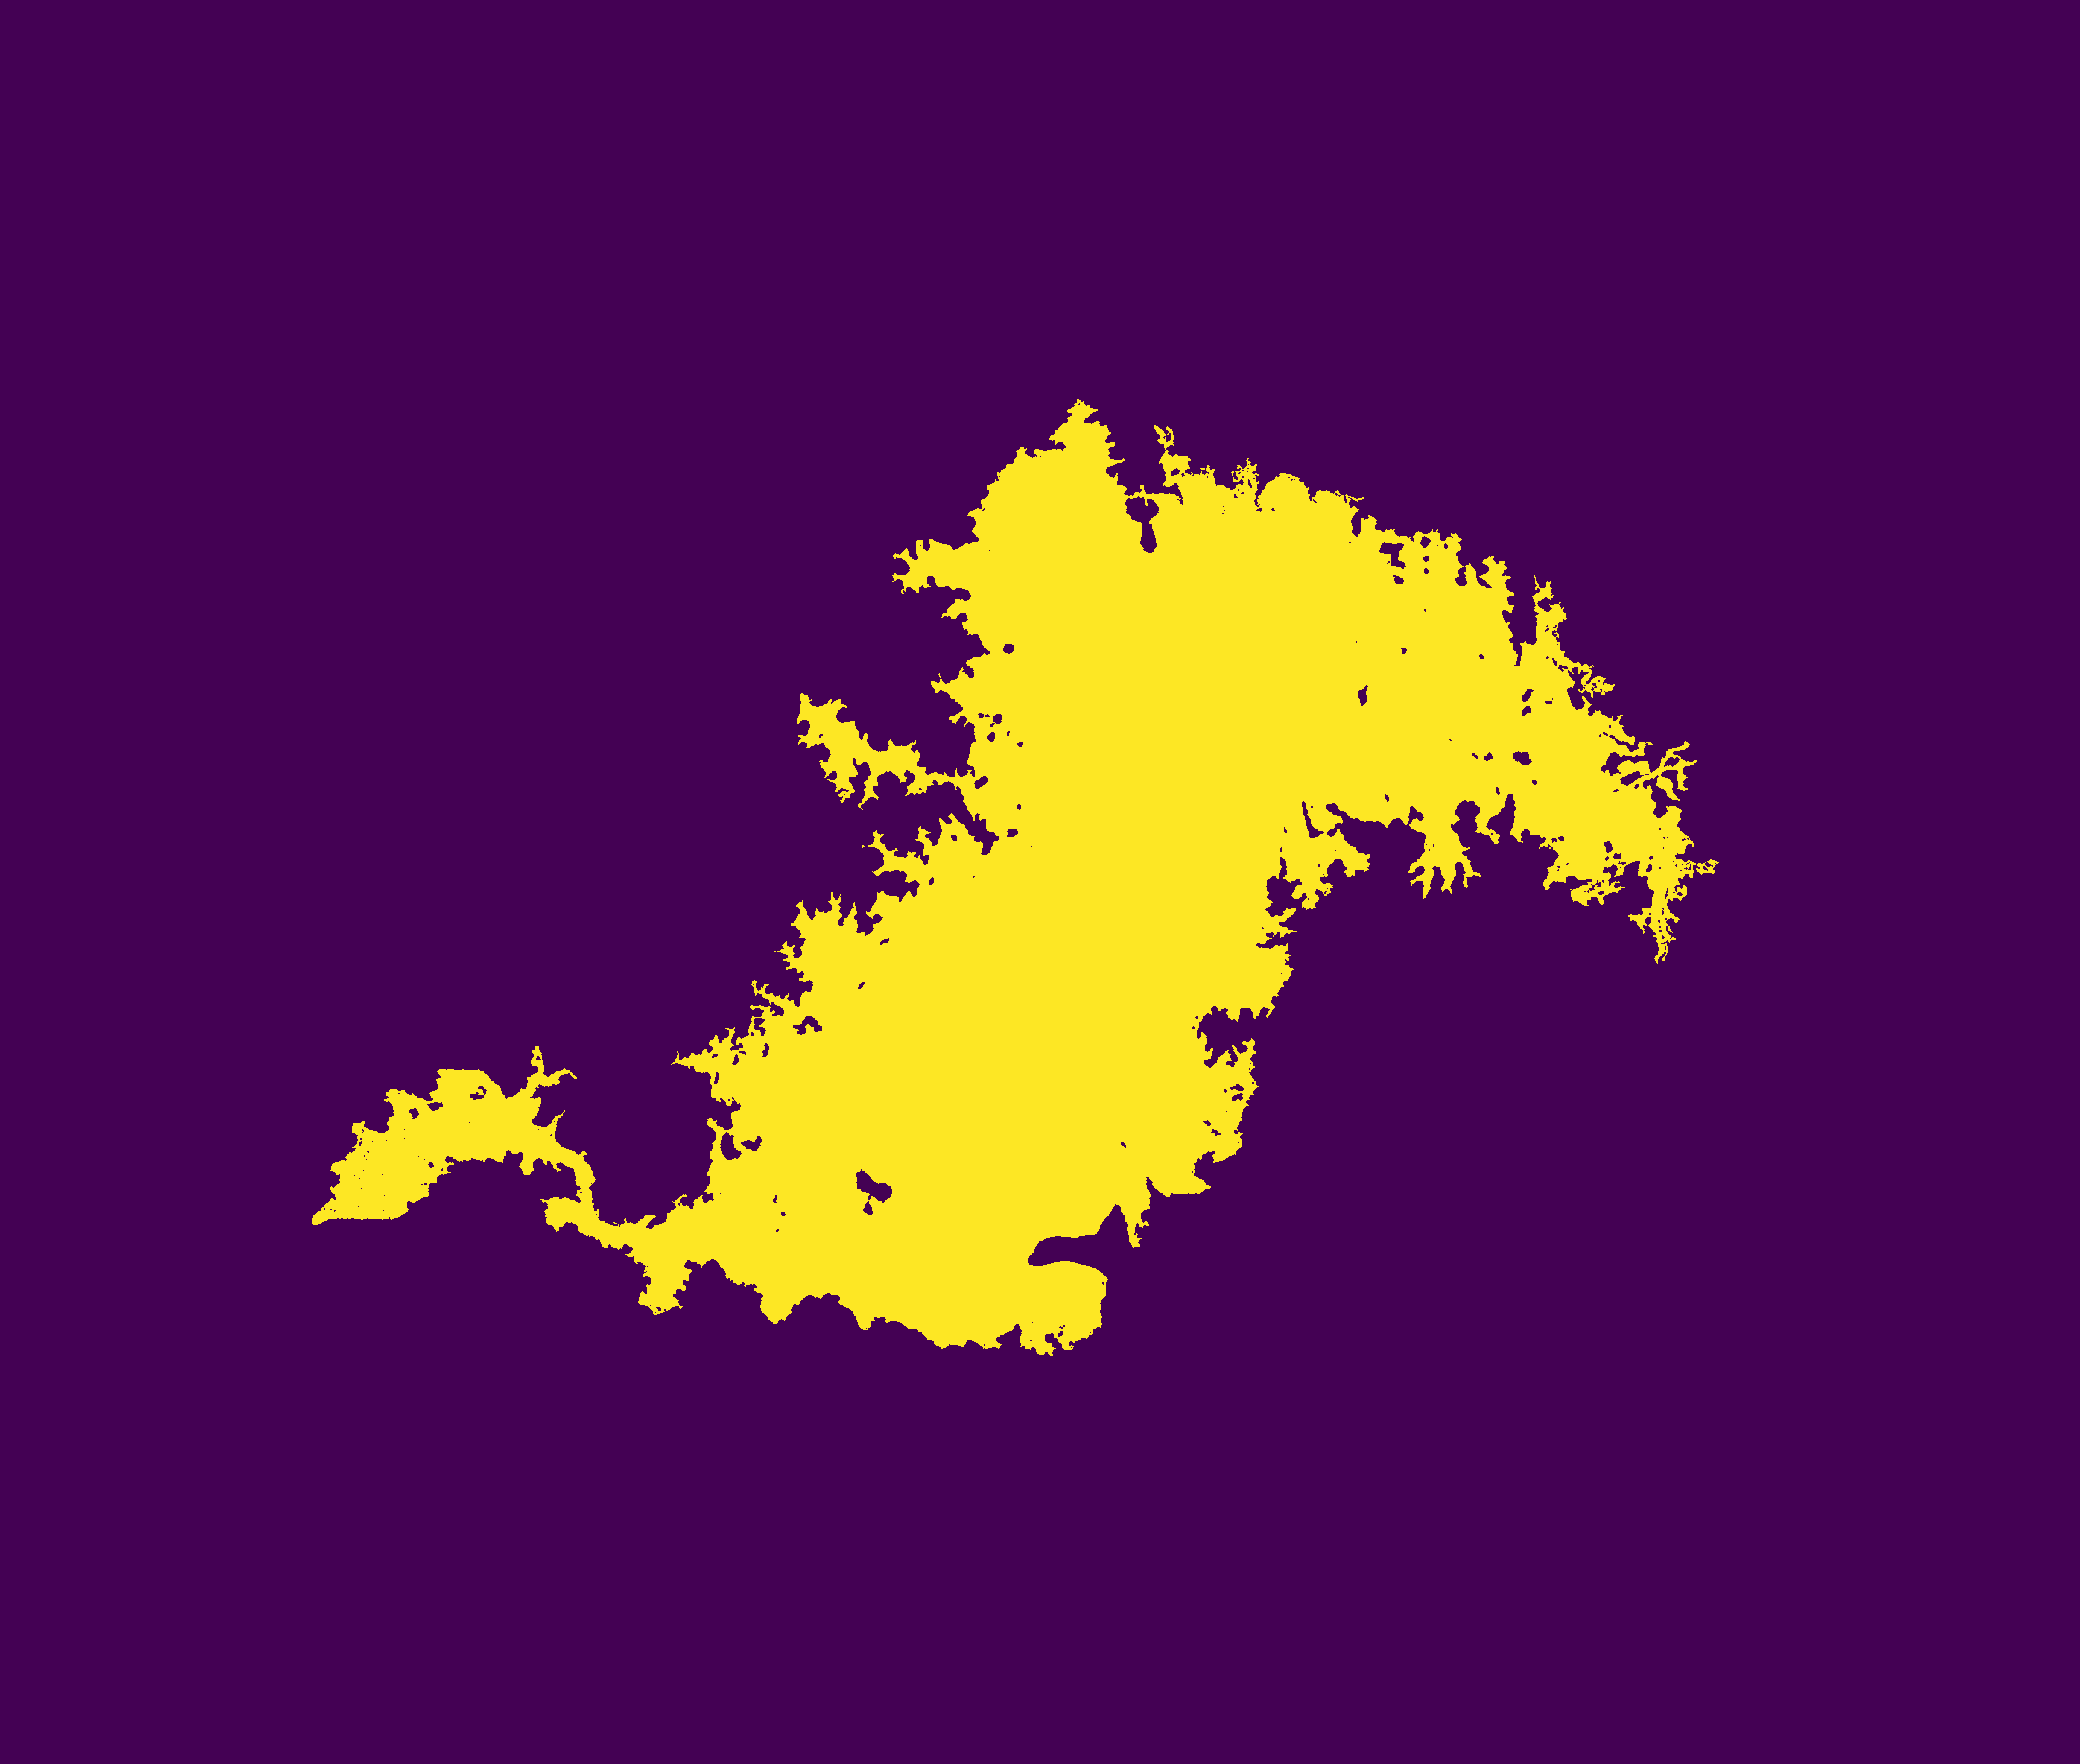
\includegraphics[width=0.32\linewidth]{figures/20170730_258_6828.png}
} 

\centering
\caption{
	\textbf{(a, b)} Landsat 8, Aug 2nd, 2017.
	\textbf{(c)} Sentinel-1, Jul 30th, 2017.}
\end{figure}

\subsection{Experiments on time-series data}

\subsubsection{Easiest case: Simple cloud shape}

\begin{figure}[]
	\centering
	\subfloat[]{
		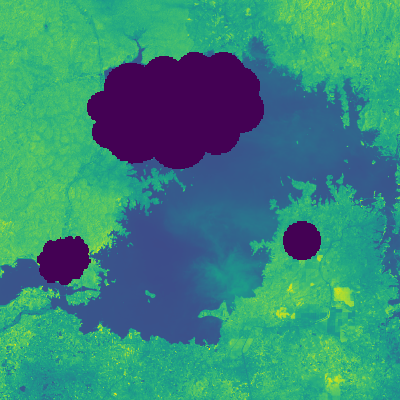
\includegraphics[width=0.24\linewidth]{figures/cont5_masked.png}
	}
	\subfloat[]{
		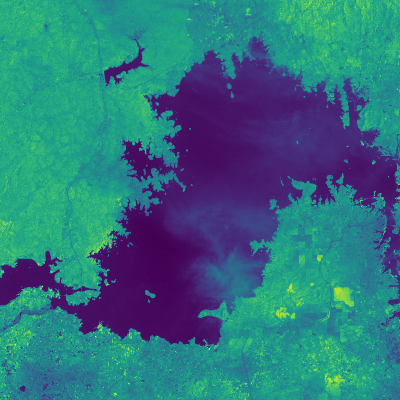
\includegraphics[width=0.24\linewidth]{figures/cont5_gt.png}
	}
	\subfloat[]{
		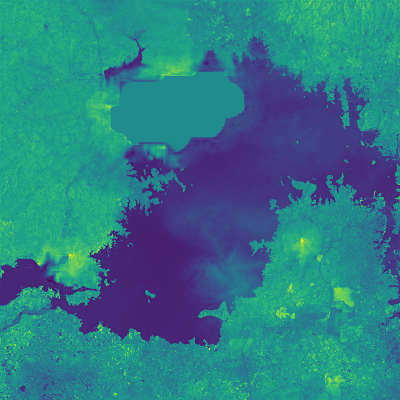
\includegraphics[width=0.24\linewidth]{figures/rcnn_simple.png}
	}
	\subfloat[]{
		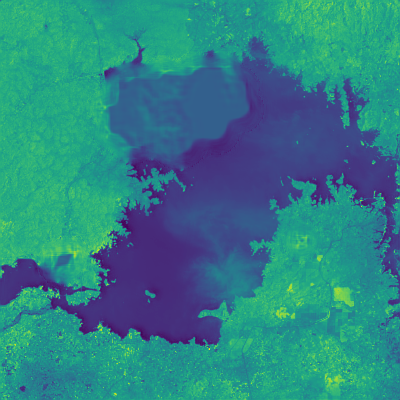
\includegraphics[width=0.24\linewidth]{figures/timecnn_simple.png}
	}  
	\centering
	\caption{Some clouds with simple shape}
\end{figure}

The result shows that for small regions, both methods could work well, but for a large missing region, it's not easy to get information from time-series images for recovery. Despite higher result in $PSNR$ metric, the recovered region by time-series images look worse than the single image as reference.

\subsubsection{Average case: Multi-simple cloud shape}

\begin{figure}[]
	\centering
	\subfloat[]{
		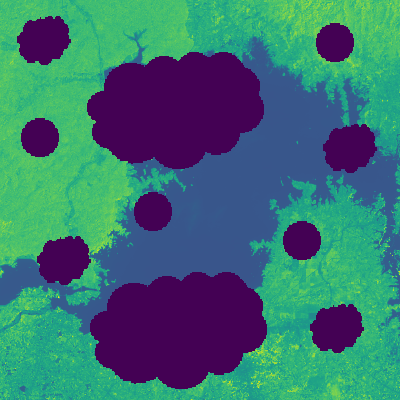
\includegraphics[width=0.24\linewidth]{figures/med_1.png}
	}
	\subfloat[]{
		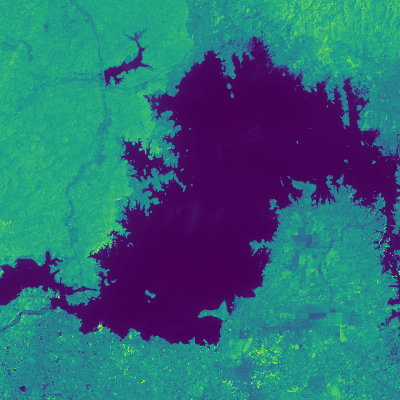
\includegraphics[width=0.24\linewidth]{figures/med_2.png}
	}
	\subfloat[]{
		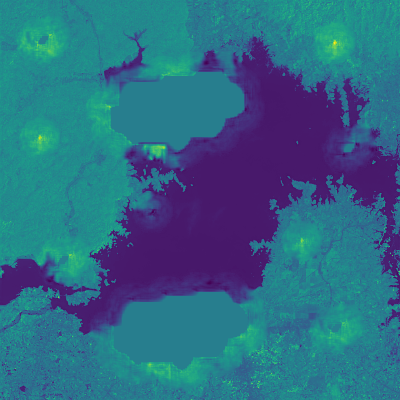
\includegraphics[width=0.24\linewidth]{figures/rcnn_med.png}
	}
	\subfloat[]{
		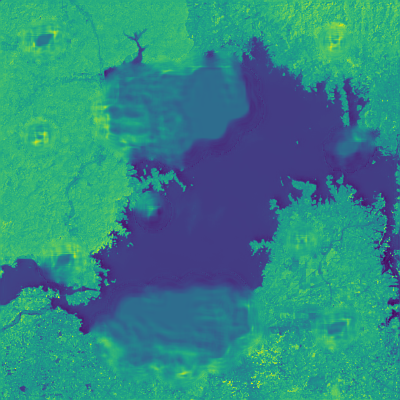
\includegraphics[width=0.24\linewidth]{figures/timecnn_med.png}
	}  
	\centering
	\caption{The result many clouds, in simple shape}
\end{figure}

\subsubsection{Hardest case: Real cloud}

\begin{figure}[]
	\centering
	\subfloat[]{
		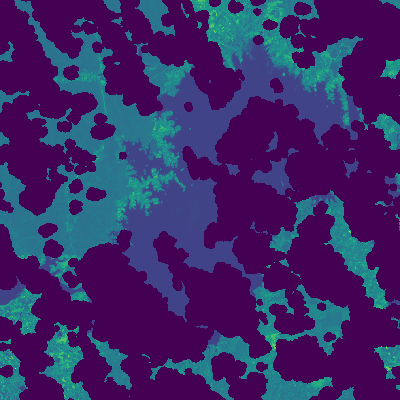
\includegraphics[width=0.24\linewidth]{figures/complext_1.png}
	}
	\subfloat[]{
		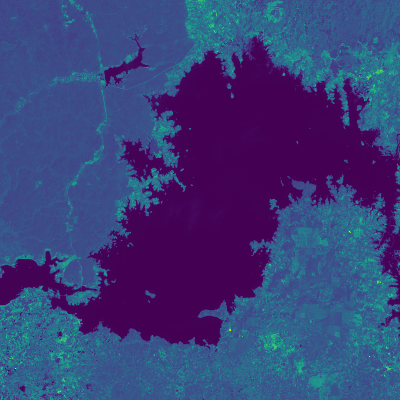
\includegraphics[width=0.24\linewidth]{figures/complext_2.png}
	}
	\subfloat[]{
		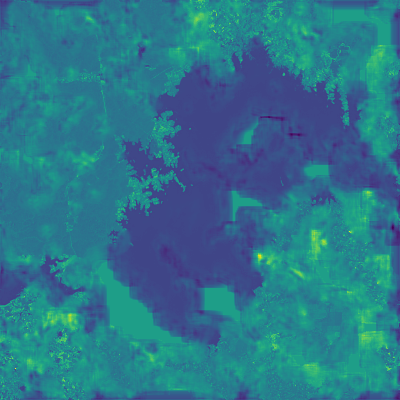
\includegraphics[width=0.24\linewidth]{figures/rcnn_complex.png}
	}
	\subfloat[]{
		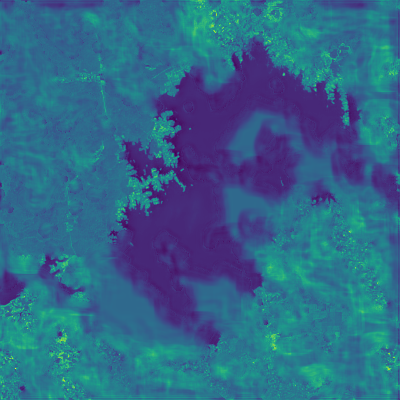
\includegraphics[width=0.24\linewidth]{figures/timecnn_complex.png}
	}  
	\centering
	\caption{The result on the most complex situation: Real cloud}
\end{figure}

\section{Conclusions}

For optimizing existing method: Scale image to range of $0..1$ slightly get better result than $0..255$. For range of $0..1$, $PSNR$ can be calculated faster as following, because $MAX_I = 1$, so $log_{10}(MAX_I) \textrm{ = } 0$ :

\begin{equation}
\centering
PSNR \textrm{ = } 20 * log_{10}(MAX_I) - 10 * log_{10}(MSE) \textrm{ = } -10 * log_{10}(MSE)
\end{equation}

Seemed to be more complex than original method, the modified model gives better result all over cases. Beside adding more one input to model, we've changed kernel filter of some layers. For some experiments, we found that larger kernel filter size gives better result, but adding more Convolutional layers doesn't. This looks like what mentioned in \textit{Image Super-Resolution Using Deep Convolutional Networks}, Chao et al.

Although the result of reconstruction is quite good when compare to existing method, when taking experiments on real images, it is not as good as expected. It might be quite good if only use it for a look. However, the model could be improved by not resizing the image to $400x400$ size. We could split it to tiles of $400x400$. It is not only keeping the original size, but also keeping details of original images, which is very good for training model.

The result of experiments on time-series images are not as good as expected. Firstly, the input as references for recovery part in network is only one (for a methods in \textbf{Chapter 3.2}, it is two). The second is, the sub-network for prediction is too simple. Itself is a very difficult problem. It is quite similar to a \textit{Moving MNIST problems}, for visualization, see at \href{http://www.cs.toronto.edu/~nitish/unsupervised_video/}{Department of Computer Science, Toronto University}. Some of papers has mentioned about it, for example, \textbf{Convolutional LSTM Network: A Machine Learning Approach for Precipitation Nowcasting}, Xingjian et al. So that, this sub-network have to be considered more complex. 